% Options for packages loaded elsewhere
% Options for packages loaded elsewhere
\PassOptionsToPackage{unicode}{hyperref}
\PassOptionsToPackage{hyphens}{url}
\PassOptionsToPackage{dvipsnames,svgnames,x11names}{xcolor}
%
\documentclass[
]{article}
\usepackage{xcolor}
\usepackage{amsmath,amssymb}
\setcounter{secnumdepth}{-\maxdimen} % remove section numbering
\usepackage{iftex}
\ifPDFTeX
  \usepackage[T1]{fontenc}
  \usepackage[utf8]{inputenc}
  \usepackage{textcomp} % provide euro and other symbols
\else % if luatex or xetex
  \usepackage{unicode-math} % this also loads fontspec
  \defaultfontfeatures{Scale=MatchLowercase}
  \defaultfontfeatures[\rmfamily]{Ligatures=TeX,Scale=1}
\fi
\usepackage{lmodern}
\ifPDFTeX\else
  % xetex/luatex font selection
\fi
% Use upquote if available, for straight quotes in verbatim environments
\IfFileExists{upquote.sty}{\usepackage{upquote}}{}
\IfFileExists{microtype.sty}{% use microtype if available
  \usepackage[]{microtype}
  \UseMicrotypeSet[protrusion]{basicmath} % disable protrusion for tt fonts
}{}
\makeatletter
\@ifundefined{KOMAClassName}{% if non-KOMA class
  \IfFileExists{parskip.sty}{%
    \usepackage{parskip}
  }{% else
    \setlength{\parindent}{0pt}
    \setlength{\parskip}{6pt plus 2pt minus 1pt}}
}{% if KOMA class
  \KOMAoptions{parskip=half}}
\makeatother
% Make \paragraph and \subparagraph free-standing
\makeatletter
\ifx\paragraph\undefined\else
  \let\oldparagraph\paragraph
  \renewcommand{\paragraph}{
    \@ifstar
      \xxxParagraphStar
      \xxxParagraphNoStar
  }
  \newcommand{\xxxParagraphStar}[1]{\oldparagraph*{#1}\mbox{}}
  \newcommand{\xxxParagraphNoStar}[1]{\oldparagraph{#1}\mbox{}}
\fi
\ifx\subparagraph\undefined\else
  \let\oldsubparagraph\subparagraph
  \renewcommand{\subparagraph}{
    \@ifstar
      \xxxSubParagraphStar
      \xxxSubParagraphNoStar
  }
  \newcommand{\xxxSubParagraphStar}[1]{\oldsubparagraph*{#1}\mbox{}}
  \newcommand{\xxxSubParagraphNoStar}[1]{\oldsubparagraph{#1}\mbox{}}
\fi
\makeatother

\usepackage{color}
\usepackage{fancyvrb}
\newcommand{\VerbBar}{|}
\newcommand{\VERB}{\Verb[commandchars=\\\{\}]}
\DefineVerbatimEnvironment{Highlighting}{Verbatim}{commandchars=\\\{\}}
% Add ',fontsize=\small' for more characters per line
\usepackage{framed}
\definecolor{shadecolor}{RGB}{241,243,245}
\newenvironment{Shaded}{\begin{snugshade}}{\end{snugshade}}
\newcommand{\AlertTok}[1]{\textcolor[rgb]{0.68,0.00,0.00}{#1}}
\newcommand{\AnnotationTok}[1]{\textcolor[rgb]{0.37,0.37,0.37}{#1}}
\newcommand{\AttributeTok}[1]{\textcolor[rgb]{0.40,0.45,0.13}{#1}}
\newcommand{\BaseNTok}[1]{\textcolor[rgb]{0.68,0.00,0.00}{#1}}
\newcommand{\BuiltInTok}[1]{\textcolor[rgb]{0.00,0.23,0.31}{#1}}
\newcommand{\CharTok}[1]{\textcolor[rgb]{0.13,0.47,0.30}{#1}}
\newcommand{\CommentTok}[1]{\textcolor[rgb]{0.37,0.37,0.37}{#1}}
\newcommand{\CommentVarTok}[1]{\textcolor[rgb]{0.37,0.37,0.37}{\textit{#1}}}
\newcommand{\ConstantTok}[1]{\textcolor[rgb]{0.56,0.35,0.01}{#1}}
\newcommand{\ControlFlowTok}[1]{\textcolor[rgb]{0.00,0.23,0.31}{\textbf{#1}}}
\newcommand{\DataTypeTok}[1]{\textcolor[rgb]{0.68,0.00,0.00}{#1}}
\newcommand{\DecValTok}[1]{\textcolor[rgb]{0.68,0.00,0.00}{#1}}
\newcommand{\DocumentationTok}[1]{\textcolor[rgb]{0.37,0.37,0.37}{\textit{#1}}}
\newcommand{\ErrorTok}[1]{\textcolor[rgb]{0.68,0.00,0.00}{#1}}
\newcommand{\ExtensionTok}[1]{\textcolor[rgb]{0.00,0.23,0.31}{#1}}
\newcommand{\FloatTok}[1]{\textcolor[rgb]{0.68,0.00,0.00}{#1}}
\newcommand{\FunctionTok}[1]{\textcolor[rgb]{0.28,0.35,0.67}{#1}}
\newcommand{\ImportTok}[1]{\textcolor[rgb]{0.00,0.46,0.62}{#1}}
\newcommand{\InformationTok}[1]{\textcolor[rgb]{0.37,0.37,0.37}{#1}}
\newcommand{\KeywordTok}[1]{\textcolor[rgb]{0.00,0.23,0.31}{\textbf{#1}}}
\newcommand{\NormalTok}[1]{\textcolor[rgb]{0.00,0.23,0.31}{#1}}
\newcommand{\OperatorTok}[1]{\textcolor[rgb]{0.37,0.37,0.37}{#1}}
\newcommand{\OtherTok}[1]{\textcolor[rgb]{0.00,0.23,0.31}{#1}}
\newcommand{\PreprocessorTok}[1]{\textcolor[rgb]{0.68,0.00,0.00}{#1}}
\newcommand{\RegionMarkerTok}[1]{\textcolor[rgb]{0.00,0.23,0.31}{#1}}
\newcommand{\SpecialCharTok}[1]{\textcolor[rgb]{0.37,0.37,0.37}{#1}}
\newcommand{\SpecialStringTok}[1]{\textcolor[rgb]{0.13,0.47,0.30}{#1}}
\newcommand{\StringTok}[1]{\textcolor[rgb]{0.13,0.47,0.30}{#1}}
\newcommand{\VariableTok}[1]{\textcolor[rgb]{0.07,0.07,0.07}{#1}}
\newcommand{\VerbatimStringTok}[1]{\textcolor[rgb]{0.13,0.47,0.30}{#1}}
\newcommand{\WarningTok}[1]{\textcolor[rgb]{0.37,0.37,0.37}{\textit{#1}}}

\providecommand{\tightlist}{%
  \setlength{\itemsep}{0pt}\setlength{\parskip}{0pt}}\usepackage{longtable,booktabs,array}
\usepackage{calc} % for calculating minipage widths
% Correct order of tables after \paragraph or \subparagraph
\usepackage{etoolbox}
\makeatletter
\patchcmd\longtable{\par}{\if@noskipsec\mbox{}\fi\par}{}{}
\makeatother
% Allow footnotes in longtable head/foot
\IfFileExists{footnotehyper.sty}{\usepackage{footnotehyper}}{\usepackage{footnote}}
\makesavenoteenv{longtable}
\usepackage{graphicx}
\makeatletter
\newsavebox\pandoc@box
\newcommand*\pandocbounded[1]{% scales image to fit in text height/width
  \sbox\pandoc@box{#1}%
  \Gscale@div\@tempa{\textheight}{\dimexpr\ht\pandoc@box+\dp\pandoc@box\relax}%
  \Gscale@div\@tempb{\linewidth}{\wd\pandoc@box}%
  \ifdim\@tempb\p@<\@tempa\p@\let\@tempa\@tempb\fi% select the smaller of both
  \ifdim\@tempa\p@<\p@\scalebox{\@tempa}{\usebox\pandoc@box}%
  \else\usebox{\pandoc@box}%
  \fi%
}
% Set default figure placement to htbp
\def\fps@figure{htbp}
\makeatother

\makeatletter
\@ifpackageloaded{float}{}{\usepackage{float}}
\floatstyle{plain}
\@ifundefined{c@chapter}{\newfloat{vid}{h}{lovid}}{\newfloat{vid}{h}{lovid}[chapter]}
\floatname{vid}{Video}
\newcommand*\listofvids{\listof{vid}{List of Videos}}
\makeatother
\makeatletter
\@ifpackageloaded{caption}{}{\usepackage{caption}}
\AtBeginDocument{%
\ifdefined\contentsname
  \renewcommand*\contentsname{Table of contents}
\else
  \newcommand\contentsname{Table of contents}
\fi
\ifdefined\listfigurename
  \renewcommand*\listfigurename{List of Figures}
\else
  \newcommand\listfigurename{List of Figures}
\fi
\ifdefined\listtablename
  \renewcommand*\listtablename{List of Tables}
\else
  \newcommand\listtablename{List of Tables}
\fi
\ifdefined\figurename
  \renewcommand*\figurename{Figure}
\else
  \newcommand\figurename{Figure}
\fi
\ifdefined\tablename
  \renewcommand*\tablename{Table}
\else
  \newcommand\tablename{Table}
\fi
}
\@ifpackageloaded{float}{}{\usepackage{float}}
\floatstyle{ruled}
\@ifundefined{c@chapter}{\newfloat{codelisting}{h}{lop}}{\newfloat{codelisting}{h}{lop}[chapter]}
\floatname{codelisting}{Listing}
\newcommand*\listoflistings{\listof{codelisting}{List of Listings}}
\makeatother
\makeatletter
\makeatother
\makeatletter
\@ifpackageloaded{caption}{}{\usepackage{caption}}
\@ifpackageloaded{subcaption}{}{\usepackage{subcaption}}
\makeatother
\newcommand{\fbxIconPath}{../../../../assets/images/icons/callouts}
\newcommand{\fbxIconFormat}{png}
\makeatletter
\@ifpackageloaded{tcolorbox}{}{\usepackage[many]{tcolorbox}}
\makeatother
%%%% ---foldboxy preamble ----- %%%%%

% Icon path and format configuration - can be overridden in filter-metadata
\providecommand{\fbxIconPath}{assets/images/icons/callouts}
\providecommand{\fbxIconFormat}{pdf}

% Legacy fallback colors (keep for compatibility)
\definecolor{fbx-default-color1}{HTML}{c7c7d0}
\definecolor{fbx-default-color2}{HTML}{a3a3aa}
\definecolor{fbox-color1}{HTML}{c7c7d0}
\definecolor{fbox-color2}{HTML}{a3a3aa}

% arguments: #1 typelabelnummer: #2 titel: #3
\newenvironment{fbx}[3]{%
\begin{tcolorbox}[
  enhanced,
  breakable,
  %fontupper=\fontsize{8pt}{10}\selectfont,
  before skip=8pt,  % space above box (increased)
  after skip=8pt,   % space below box (increased)
  attach boxed title to top*={xshift=0pt},
  boxed title style={
  %fuzzy shadow={1pt}{-1pt}{0mm}{0.1mm}{gray},
  arc=1.5pt,
  rounded corners=north,
  sharp corners=south,
  top=6pt,          % Adjusted for ~40px equivalent height
  bottom=5pt,       % Adjusted for ~40px equivalent height
  overlay={
      \node [left,outer sep=0em, black,draw=none,anchor=west,
        rectangle,fill=none,inner sep=0pt]
        at ([xshift=4mm]frame.west) {\includegraphics[width=4.2mm]{\fbxIconPath/icon_#1.\fbxIconFormat}};
    },
  },
  colframe=#1-color2,             % Border color (auto-generated from YAML)
  colbacktitle=#1-color1,         % Background color (auto-generated from YAML)
  colback=white,
  coltitle=black,
  titlerule=0mm,
  toprule=0.5pt,
  bottomrule=0.5pt,
  leftrule=2.2pt,
  rightrule=0.5pt,
  outer arc=1.5pt,
  arc=1.5pt,
  left=0.5em,       % increased left padding
  bottomtitle=1.5mm, % increased title bottom margin
  toptitle=1.5mm,    % increased title top margin
  title=\hspace{2.5em}{#2}\hspace{0.2em}{#3}, % Removed \textbf for normal weight
  extras middle and last={top=4pt} % increased continuation spacing
]}
{\end{tcolorbox}}


% boxed environment with right border
\newenvironment{fbxSimple}[3]{\begin{tcolorbox}[
  enhanced,
  breakable,
  %fontupper=\fontsize{8pt}{10}\selectfont,
  before skip=8pt,  % space above box (increased)
  after skip=8pt,   % space below box (increased)
  attach boxed title to top*={xshift=0pt},
  boxed title style={
  %fuzzy shadow={1pt}{-1pt}{0mm}{0.1mm}{gray},
  arc=1.5pt,
  rounded corners=north,
  sharp corners=south,
  top=6pt,          % Adjusted for ~40px equivalent height
  bottom=5pt,       % Adjusted for ~40px equivalent height
  overlay={
      \node [left,outer sep=0em, black,draw=none,anchor=west,
        rectangle,fill=none,inner sep=0pt]
        at ([xshift=3mm]frame.west) {\includegraphics[width=4.2mm]{\fbxIconPath/icon_#1.\fbxIconFormat}};
    },
  },
  colframe=#1-color2,             % Border color (auto-generated from YAML)
  colbacktitle=#1-color1,         % Background color (auto-generated from YAML)
  colback=white,
  coltitle=black,
  titlerule=0mm,
  toprule=0.5pt,
  bottomrule=0.5pt,
  leftrule=2.2pt,
  rightrule=0.5pt,
  outer arc=1.5pt,
  arc=1.5pt,
  left=0.5em,       % increased left padding
  bottomtitle=1.5mm, % increased title bottom margin
  toptitle=1.5mm,    % increased title top margin
  title=\hspace{2.5em}{#2}\hspace{0.2em}{#3}, % Removed \textbf for normal weight
  boxsep=1pt,
  extras first={bottom=0pt},
  extras last={top=0pt,bottom=1pt},
  overlay first={
    \draw[line width=1pt,white] ([xshift=2.2pt]frame.south west)-- ([xshift=-0.5pt]frame.south east);
  },
  overlay last={
    \draw[line width=1pt,white] ([xshift=2.2pt]frame.north west)-- ([xshift=-0.5pt]frame.north east);
   }
]}
{\end{tcolorbox}}

%%%% --- end foldboxy preamble ----- %%%%% 
%%==== colors from yaml ===%
\definecolor{callout-resource-videos-color1}{HTML}{E0F2F1}
\definecolor{callout-resource-videos-color2}{HTML}{20B2AA}
\definecolor{callout-quiz-question-color1}{HTML}{F0F0F8}
\definecolor{callout-quiz-question-color2}{HTML}{5B4B8A}
\definecolor{callout-resource-slides-color1}{HTML}{E0F2F1}
\definecolor{callout-resource-slides-color2}{HTML}{20B2AA}
\definecolor{callout-resource-exercises-color1}{HTML}{E0F2F1}
\definecolor{callout-resource-exercises-color2}{HTML}{20B2AA}
\definecolor{callout-code-color1}{HTML}{F2F4F8}
\definecolor{callout-code-color2}{HTML}{D1D7E0}
\definecolor{callout-quiz-answer-color1}{HTML}{E8F2EA}
\definecolor{callout-quiz-answer-color2}{HTML}{4a7c59}
\definecolor{callout-chapter-connection-color1}{HTML}{FDF2F7}
\definecolor{callout-chapter-connection-color2}{HTML}{A51C30}
%=============%

\usepackage{hyphenat}
\usepackage{ifthen}
\usepackage{calc}
\usepackage{calculator}



\usepackage{graphicx}
\usepackage{geometry}
\usepackage{afterpage}
\usepackage{tikz}
\usetikzlibrary{calc}
\usetikzlibrary{fadings}
\usepackage[pagecolor=none]{pagecolor}


% Set the titlepage font families







% Set the coverpage font families

\usepackage{bookmark}
\IfFileExists{xurl.sty}{\usepackage{xurl}}{} % add URL line breaks if available
\urlstyle{same}
\hypersetup{
  colorlinks=true,
  linkcolor={blue},
  filecolor={Maroon},
  citecolor={Blue},
  urlcolor={Blue},
  pdfcreator={LaTeX via pandoc}}


\author{}
\date{}
\begin{document}
%%%%% begin titlepage extension code


\begin{titlepage}

%%% TITLE PAGE START

% Set up alignment commands
%Page
\newcommand{\titlepagepagealign}{
\ifthenelse{\equal{left}{right}}{\raggedleft}{}
\ifthenelse{\equal{left}{center}}{\centering}{}
\ifthenelse{\equal{left}{left}}{\raggedright}{}
}


\newcommand{\titleandsubtitle}{
% Title and subtitle
}
\newcommand{\titlepagetitleblock}{
\titleandsubtitle
}

\newcommand{\authorstyle}[1]{{#1}}

\newcommand{\affiliationstyle}[1]{{#1}}

\newcommand{\titlepageauthorblock}{
{\authorstyle{}}}

\newcommand{\titlepageaffiliationblock}{
\hangindent=1em
\hangafter=1
{\affiliationstyle{


\vspace{1\baselineskip} 
}}
}
\newcommand{\headerstyled}{%
{}
}
\newcommand{\footerstyled}{%
{}
}
\newcommand{\datestyled}{%
{}
}


\newcommand{\titlepageheaderblock}{\headerstyled}

\newcommand{\titlepagefooterblock}{
\footerstyled
}

\newcommand{\titlepagedateblock}{
\datestyled
}

%set up blocks so user can specify order
\newcommand{\titleblock}{}

\newcommand{\authorblock}{}

\newcommand{\affiliationblock}{}

\newcommand{\logoblock}{}

\newcommand{\footerblock}{}

\newcommand{\dateblock}{}

\newcommand{\headerblock}{}

\thispagestyle{empty} % no page numbers on titlepages


\newlength{\minipagewidth}
\setlength{\minipagewidth}{\textwidth}
\raggedright % single minipage
% [position of box][box height][inner position]{width}
% [s] means stretch out vertically; assuming there is a vfill
\begin{minipage}[b][\textheight][s]{\minipagewidth}
\titlepagepagealign
\headerblock

\titleblock

\authorblock

\affiliationblock

\vfill

\logoblock

\footerblock
\par

\end{minipage}\ifthenelse{\equal{}{right} \OR \equal{}{leftright} }{
\hspace{\B}
\vrulecode}{}
\clearpage
%%% TITLE PAGE END
\end{titlepage}
\setcounter{page}{1}

%%%%% end titlepage extension code


\section*{Setup}\label{setup}
\addcontentsline{toc}{section}{Setup}

\begin{figure}[H]

{\centering \pandocbounded{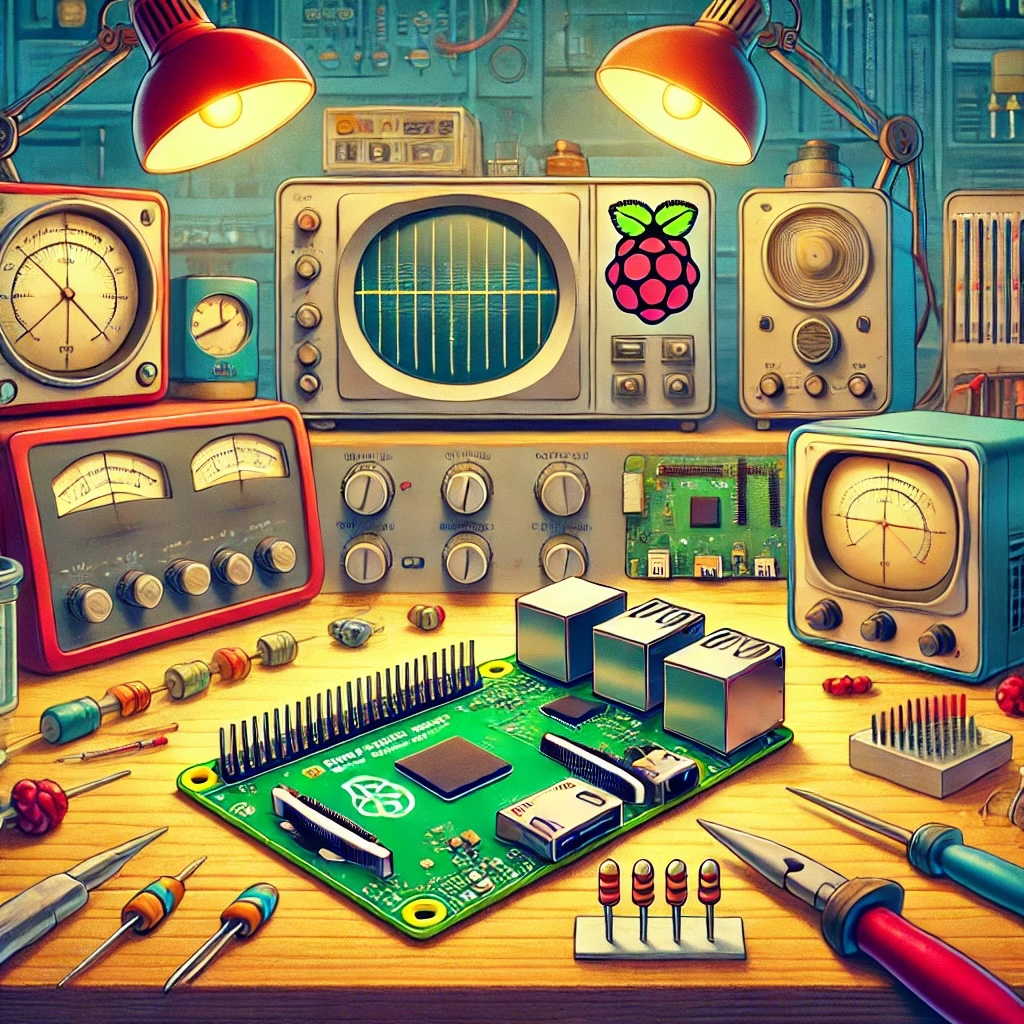
\includegraphics[keepaspectratio]{images/jpeg/rasp_setup_portada.jpg}}

}

\caption{\emph{DALL·E prompt - An electronics laboratory environment
inspired by the 1950s, with a cartoon style. The lab should have vintage
equipment, large oscilloscopes, old-fashioned tube radios, and large,
boxy computers. The Raspberry Pi 5 board is prominently displayed,
accurately shown in its real size, similar to a credit card, on a
workbench. The Pi board is surrounded by classic lab tools like a
soldering iron, resistors, and wires. The overall scene should be
vibrant, with exaggerated colors and playful details characteristic of a
cartoon. No logos or text should be included.}}

\end{figure}%

This chapter will guide you through setting up Raspberry Pi Zero 2 W
(\emph{Raspi-Zero}) and Raspberry Pi 5 (\emph{Raspi-5}) models. We'll
cover hardware setup, operating system installation, initial
configuration, and tests.

\begin{quote}
The general instructions for the \emph{Raspi-5} also apply to the older
Raspberry Pi versions, such as the Raspi-3 and Raspi-4.
\end{quote}

\subsection{Overview}\label{sec-setup-overview-737b}

The Raspberry Pi is a powerful and versatile single-board computer that
has become an essential tool for engineers across various disciplines.
Developed by the \href{https://www.raspberrypi.org/}{Raspberry Pi
Foundation}, these compact devices offer a unique combination of
affordability, computational power, and extensive GPIO (General Purpose
Input/Output) capabilities, making them ideal for prototyping, embedded
systems development, and advanced engineering projects.

\subsubsection{Key Features}\label{sec-setup-key-features-2bff}

\begin{enumerate}
\def\labelenumi{\arabic{enumi}.}
\item
  \textbf{Computational Power}: Despite their small size, Raspberry Pis
  offers significant processing capabilities, with the latest models
  featuring multi-core ARM processors and up to 8 GB of RAM.
\item
  \textbf{GPIO Interface}: The 40-pin GPIO header allows direct
  interaction with sensors, actuators, and other electronic components,
  facilitating hardware-software integration projects.
\item
  \textbf{Extensive Connectivity}: Built-in Wi-Fi, Bluetooth, Ethernet,
  and multiple USB ports enable diverse communication and networking
  projects.
\item
  \textbf{Low-Level Hardware Access}: Raspberry Pis provides access to
  interfaces like I2C, SPI, and UART, allowing for detailed control and
  communication with external devices.
\item
  \textbf{Real-Time Capabilities}: With proper configuration, Raspberry
  Pis can be used for soft real-time applications, making them suitable
  for control systems and signal processing tasks.
\item
  \textbf{Power Efficiency}: Low power consumption enables
  battery-powered and energy-efficient designs, especially in models
  like the Pi Zero.
\end{enumerate}

\subsubsection{Raspberry Pi Models (covered in this
book)}\label{sec-setup-raspberry-pi-models-covered-book-1942}

\begin{enumerate}
\def\labelenumi{\arabic{enumi}.}
\tightlist
\item
  \textbf{Raspberry Pi Zero 2 W} (\emph{Raspi-Zero}):

  \begin{itemize}
  \tightlist
  \item
    Ideal for: Compact embedded systems
  \item
    Key specs: 1 GHz single-core CPU (ARM Cortex-A53), 512 MB RAM,
    minimal power consumption
  \end{itemize}
\item
  \textbf{Raspberry Pi 5} (\emph{Raspi-5}):

  \begin{itemize}
  \tightlist
  \item
    Ideal for: More demanding applications such as edge computing,
    computer vision, and edgeAI applications, including LLMs.
  \item
    Key specs: 2.4 GHz quad-core CPU (ARM Cortex A-76), up to 8 GB RAM,
    PCIe interface for expansions
  \end{itemize}
\end{enumerate}

\subsubsection{Engineering
Applications}\label{sec-setup-engineering-applications-0b94}

\begin{enumerate}
\def\labelenumi{\arabic{enumi}.}
\item
  \textbf{Embedded Systems Design}: Develop and prototype embedded
  systems for real-world applications.
\item
  \textbf{IoT and Networked Devices}: Create interconnected devices and
  explore protocols like MQTT, CoAP, and HTTP/HTTPS.
\item
  \textbf{Control Systems}: Implement feedback control loops, PID
  controllers, and interface with actuators.
\item
  \textbf{Computer Vision and AI}: Utilize libraries like OpenCV and
  TensorFlow Lite for image processing and machine learning at the edge.
\item
  \textbf{Data Acquisition and Analysis}: Collect sensor data, perform
  real-time analysis, and create data logging systems.
\item
  \textbf{Robotics}: Build robot controllers, implement motion planning
  algorithms, and interface with motor drivers.
\item
  \textbf{Signal Processing}: Perform real-time signal analysis,
  filtering, and DSP applications.
\item
  \textbf{Network Security}: Set up VPNs, firewalls, and explore network
  penetration testing.
\end{enumerate}

This tutorial will guide you through setting up the most common
Raspberry Pi models, enabling you to start on your machine learning
project quickly. We'll cover hardware setup, operating system
installation, and initial configuration, focusing on preparing your Pi
for Machine Learning applications.

\subsection{Hardware Overview}\label{sec-setup-hardware-overview-2d2a}

\subsubsection{Raspberry Pi Zero
2W}\label{sec-setup-raspberry-pi-zero-2w-c89a}

\noindent
\pandocbounded{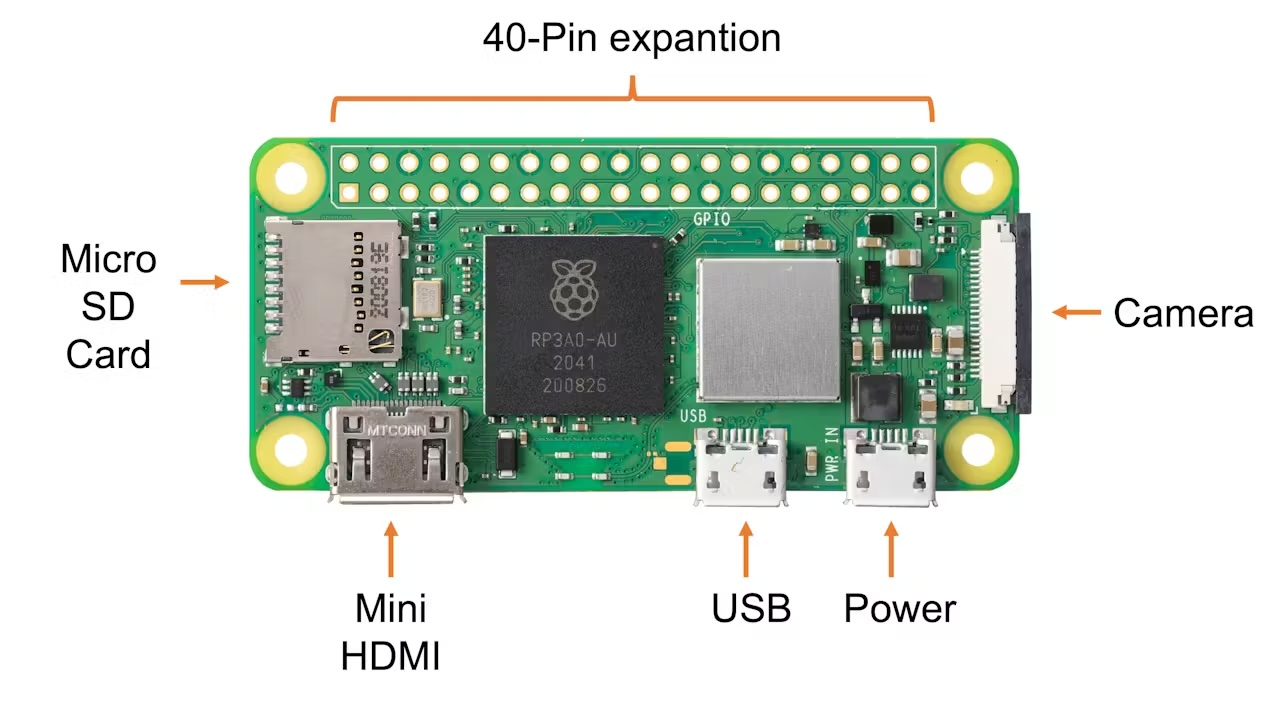
\includegraphics[keepaspectratio]{images/jpeg/zero-hardware.jpg}}

\begin{itemize}
\tightlist
\item
  \textbf{Processor}: 1 GHz quad-core 64-bit Arm Cortex-A53 CPU
\item
  \textbf{RAM}: 512 MB SDRAM
\item
  \textbf{Wireless}: 2.4 GHz 802.11 b/g/n wireless LAN, Bluetooth 4.2,
  BLE
\item
  \textbf{Ports}: Mini HDMI, micro USB OTG, CSI-2 camera connector
\item
  \textbf{Power}: 5 V via micro USB port
\end{itemize}

\subsubsection{Raspberry Pi 5}\label{sec-setup-raspberry-pi-5-f30b}

\noindent
\pandocbounded{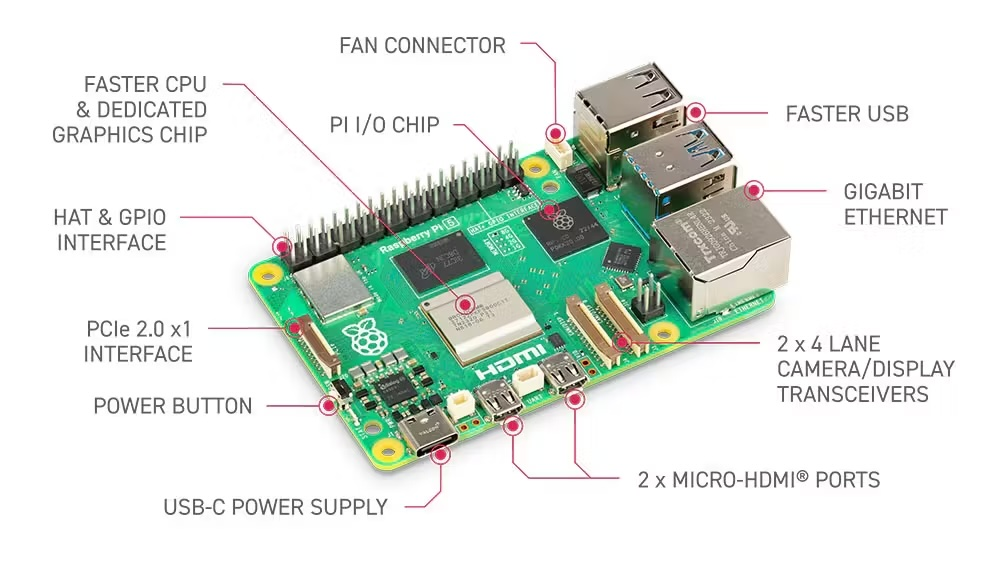
\includegraphics[keepaspectratio]{images/jpeg/r5-hardware.jpg}}

\begin{itemize}
\tightlist
\item
  \textbf{Processor}:

  \begin{itemize}
  \tightlist
  \item
    Pi 5: Quad-core 64-bit Arm Cortex-A76 CPU @ 2.4 GHz
  \item
    Pi 4: Quad-core Cortex-A72 (ARM v8) 64-bit SoC @ 1.5 GHz
  \end{itemize}
\item
  \textbf{RAM}: 2 GB, 4 GB, or 8 GB options (8 GB recommended for AI
  tasks)
\item
  \textbf{Wireless}: Dual-band 802.11ac wireless, Bluetooth 5.0
\item
  \textbf{Ports}: 2 \(\times\) micro HDMI ports, 2 \(\times\) USB 3.0
  ports, 2 \(\times\) USB 2.0 ports, CSI camera port, DSI display port
\item
  \textbf{Power}: 5 V DC via USB-C connector (3A)
\end{itemize}

\begin{quote}
In the labs, we will use different names to address the Raspberry:
\texttt{Raspi}, \texttt{Raspi-5}, \texttt{Raspi-Zero}, etc. Usually,
\texttt{Raspi} is used when the instructions or comments apply to every
model.
\end{quote}

\subsection{Installing the Operating
System}\label{sec-setup-installing-operating-system-7215}

\subsubsection{The Operating System
(OS)}\label{sec-setup-operating-system-os-2d84}

An operating system (OS) is fundamental software that manages computer
hardware and software resources, providing standard services for
computer programs. It is the core software that runs on a computer,
acting as an intermediary between hardware and application software. The
OS manages the computer's memory, processes, device drivers, files, and
security protocols.

\begin{enumerate}
\def\labelenumi{\arabic{enumi}.}
\tightlist
\item
  \textbf{Key functions}:

  \begin{itemize}
  \tightlist
  \item
    Process management: Allocating CPU time to different programs
  \item
    Memory management: Allocating and freeing up memory as needed
  \item
    File system management: Organizing and keeping track of files and
    directories
  \item
    Device management: Communicating with connected hardware devices
  \item
    User interface: Providing a way for users to interact with the
    computer
  \end{itemize}
\item
  \textbf{Components}:

  \begin{itemize}
  \tightlist
  \item
    Kernel: The core of the OS that manages hardware resources
  \item
    Shell: The user interface for interacting with the OS
  \item
    File system: Organizes and manages data storage
  \item
    Device drivers: Software that allows the OS to communicate with
    hardware
  \end{itemize}
\end{enumerate}

The Raspberry Pi runs a specialized version of Linux designed for
embedded systems. This operating system, typically a variant of Debian
called Raspberry Pi OS (formerly Raspbian), is optimized for the Pi's
ARM-based architecture and limited resources.

\begin{quote}
The latest version of Raspberry Pi OS is based on
\href{https://www.raspberrypi.com/news/bookworm-the-new-version-of-raspberry-pi-os/}{Debian
Bookworm}.
\end{quote}

\textbf{Key features}:

\begin{enumerate}
\def\labelenumi{\arabic{enumi}.}
\tightlist
\item
  Lightweight: Tailored to run efficiently on the Pi's hardware.
\item
  Versatile: Supports a wide range of applications and programming
  languages.
\item
  Open-Source: Allows for customization and community-driven
  improvements.
\item
  GPIO support: Enables interaction with sensors and other hardware
  through the Pi's pins.
\item
  Regular updates: Continuously improved for performance and security.
\end{enumerate}

Embedded Linux on the Raspberry Pi provides a full-featured operating
system in a compact package, making it ideal for projects ranging from
simple IoT devices to more complex edge machine-learning applications.
Its compatibility with standard Linux tools and libraries makes it a
powerful platform for development and experimentation.

\subsubsection{Installation}\label{sec-setup-installation-1c39}

To use the Raspberry Pi, we will need an operating system. By default,
Raspberry Pi checks for an operating system on any SD card inserted in
the slot, so we should install an operating system using
\href{https://www.raspberrypi.com/software/}{Raspberry Pi Imager.}

\emph{Raspberry Pi Imager} is a tool for downloading and writing images
on \emph{macOS}, \emph{Windows}, and \emph{Linux}. It includes many
popular operating system images for Raspberry Pi. We will also use the
Imager to preconfigure credentials and remote access settings.

Follow the steps to install the OS in your Raspi.

\begin{enumerate}
\def\labelenumi{\arabic{enumi}.}
\tightlist
\item
  \href{https://www.raspberrypi.com/software/}{Download} and install the
  Raspberry Pi Imager on your computer.
\item
  Insert a microSD card into your computer (a 32GB SD card is
  recommended) .
\item
  Open Raspberry Pi Imager and select your Raspberry Pi model.
\item
  Choose the appropriate operating system:

  \begin{itemize}
  \tightlist
  \item
    \textbf{For Raspi-Zero}: For example, you can select:
    \texttt{Raspberry\ Pi\ OS\ Lite\ (64-bit)}.
  \end{itemize}
\end{enumerate}

\noindent \begin{center}
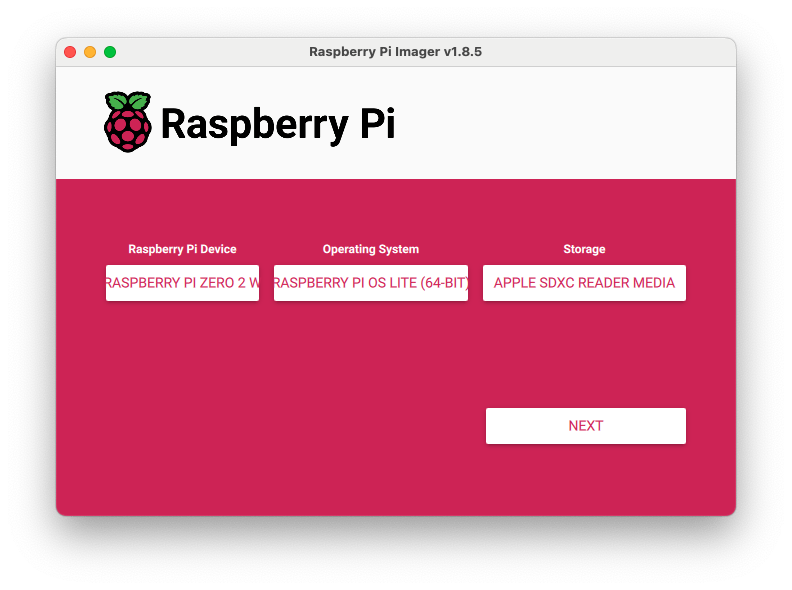
\includegraphics[width=0.7\linewidth,height=\textheight,keepaspectratio]{images/png/zero-burn.png}
\end{center}

\begin{quote}
Due to its reduced SDRAM (512 MB), the recommended OS for the Raspi-Zero
is the 32-bit version. However, to run some machine learning models,
such as the YOLOv8 from Ultralitics, we should use the 64-bit version.
Although Raspi-Zero can run a \emph{desktop}, we will choose the LITE
version (no Desktop) to reduce the RAM needed for regular operation.
\end{quote}

\begin{itemize}
\tightlist
\item
  For \textbf{Raspi-5}: We can select the full 64-bit version, which
  includes a desktop: \texttt{Raspberry\ Pi\ OS\ (64-bit)}
\end{itemize}

\noindent \begin{center}
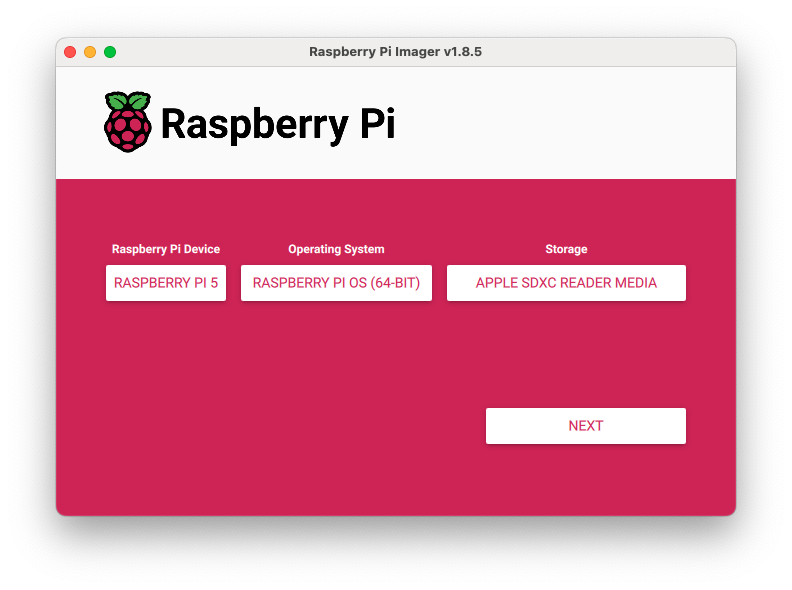
\includegraphics[width=0.7\linewidth,height=\textheight,keepaspectratio]{images/png/r5-burn.png}
\end{center}

\begin{enumerate}
\def\labelenumi{\arabic{enumi}.}
\setcounter{enumi}{4}
\tightlist
\item
  Select your microSD card as the storage device.
\item
  Click on \texttt{Next} and then the \texttt{gear} icon to access
  advanced options.
\item
  Set the \emph{hostname}, the Raspi \emph{username and password},
  configure \emph{WiFi} and \emph{enable SSH} (Very important!)
\end{enumerate}

\noindent \begin{center}
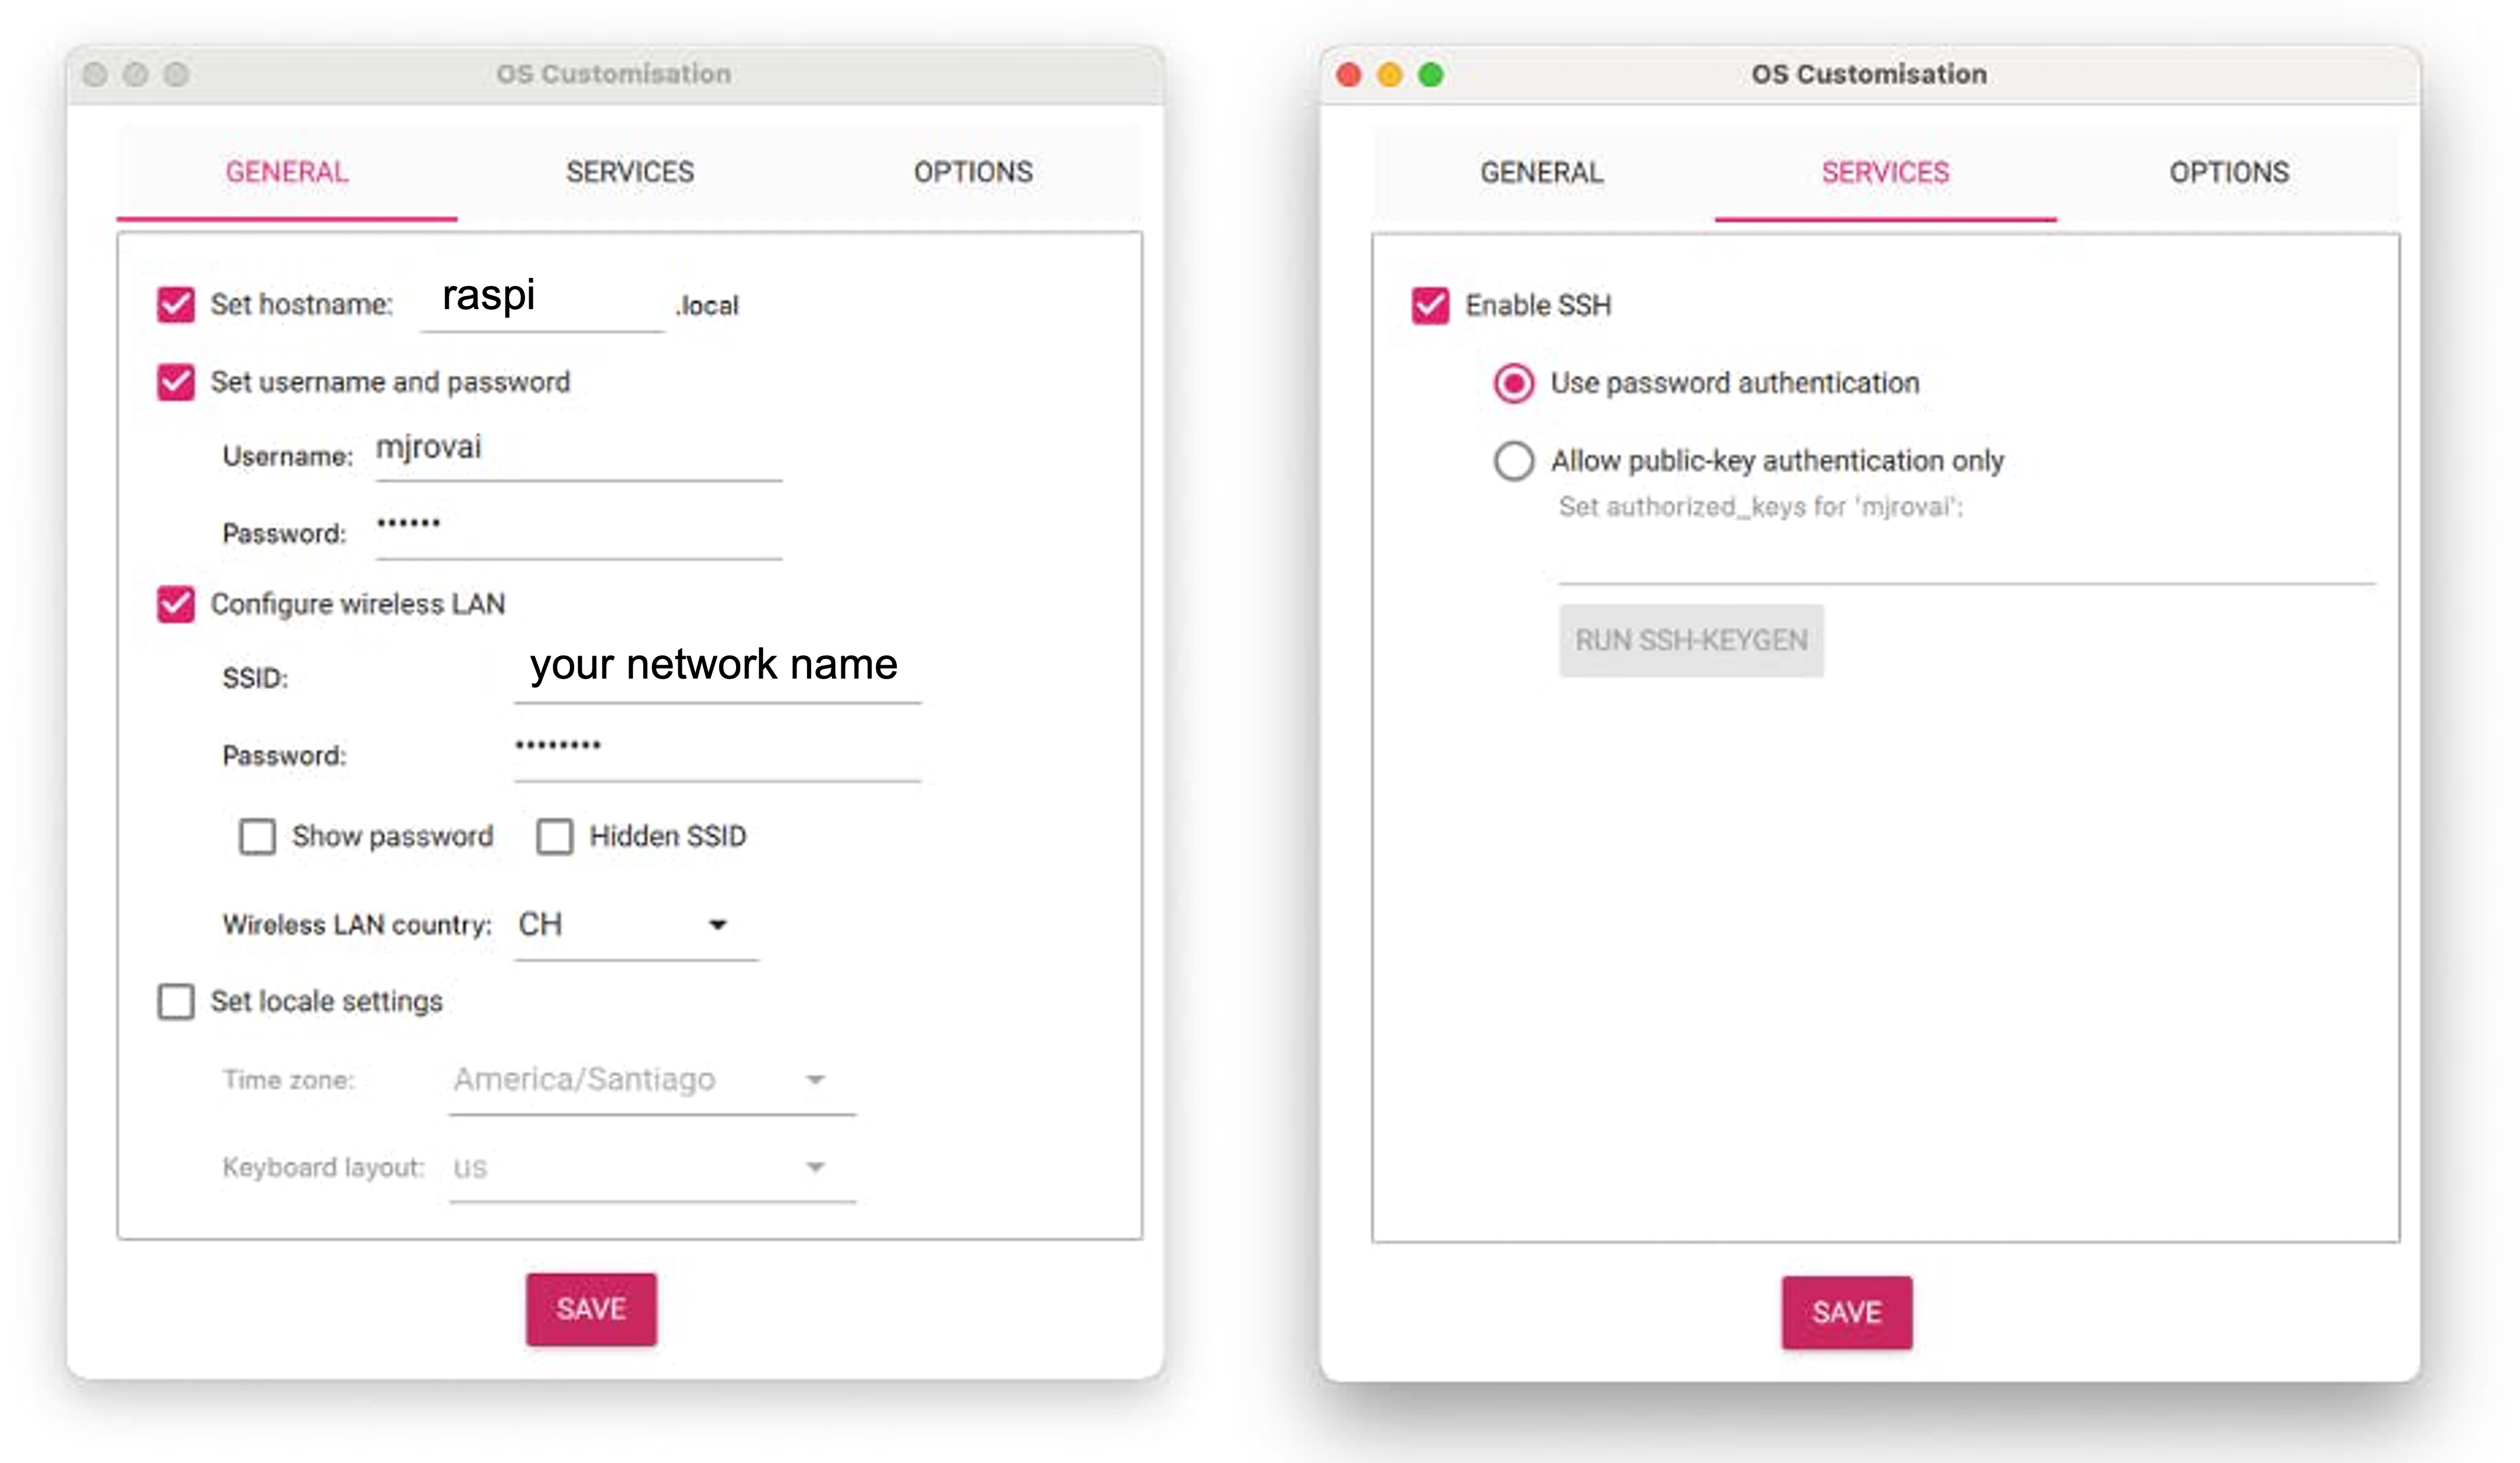
\includegraphics[width=0.9\linewidth,height=\textheight,keepaspectratio]{images/jpeg/setup.jpg}
\end{center}

\begin{enumerate}
\def\labelenumi{\arabic{enumi}.}
\setcounter{enumi}{7}
\tightlist
\item
  Write the image to the microSD card.
\end{enumerate}

\begin{quote}
In the examples here, we will use different hostnames depending on the
device used: raspi, raspi-5, raspi-Zero, etc. It would help if you
replaced it with the one you are using.
\end{quote}

\subsubsection{Initial
Configuration}\label{sec-setup-initial-configuration-c5e1}

\begin{enumerate}
\def\labelenumi{\arabic{enumi}.}
\tightlist
\item
  Insert the microSD card into your Raspberry Pi.
\item
  Connect power to boot up the Raspberry Pi.
\item
  Please wait for the initial boot process to complete (it may take a
  few minutes).
\end{enumerate}

\begin{quote}
You can find the most common Linux commands to be used with the Raspi
\href{https://www.jwdittrich.people.ysu.edu/raspberrypi/UsefulRaspberryPiCommands.pdf}{here}
or
\href{https://www.codecademy.com/learn/learn-raspberry-pi/modules/raspberry-pi-command-line-module/cheatsheet}{here}.
\end{quote}

\subsection{Remote Access}\label{sec-setup-remote-access-1a6a}

\subsubsection{SSH Access}\label{sec-setup-ssh-access-d9fd}

The easiest way to interact with the Raspi-Zero is via SSH
(``Headless''). You can use a Terminal (MAC/Linux),
\href{https://www.putty.org/}{PuTTy (}Windows), or any other.

\begin{enumerate}
\def\labelenumi{\arabic{enumi}.}
\item
  Find your Raspberry Pi's IP address (for example, check your router).
\item
  On your computer, open a terminal and connect via SSH:

\begin{Shaded}
\begin{Highlighting}[]
\FunctionTok{ssh}\NormalTok{ username@}\PreprocessorTok{[}\SpecialStringTok{raspberry\_pi\_ip\_address}\PreprocessorTok{]}
\end{Highlighting}
\end{Shaded}

  Alternatively, if you do not have the IP address, you can try the
  following: \texttt{bash\ ssh\ username@hostname.local} for example,
  \texttt{ssh\ mjrovai@rpi-5.local} , \texttt{ssh\ mjrovai@raspi.local}
  , etc.

  \begin{figure}[H]

  {\centering 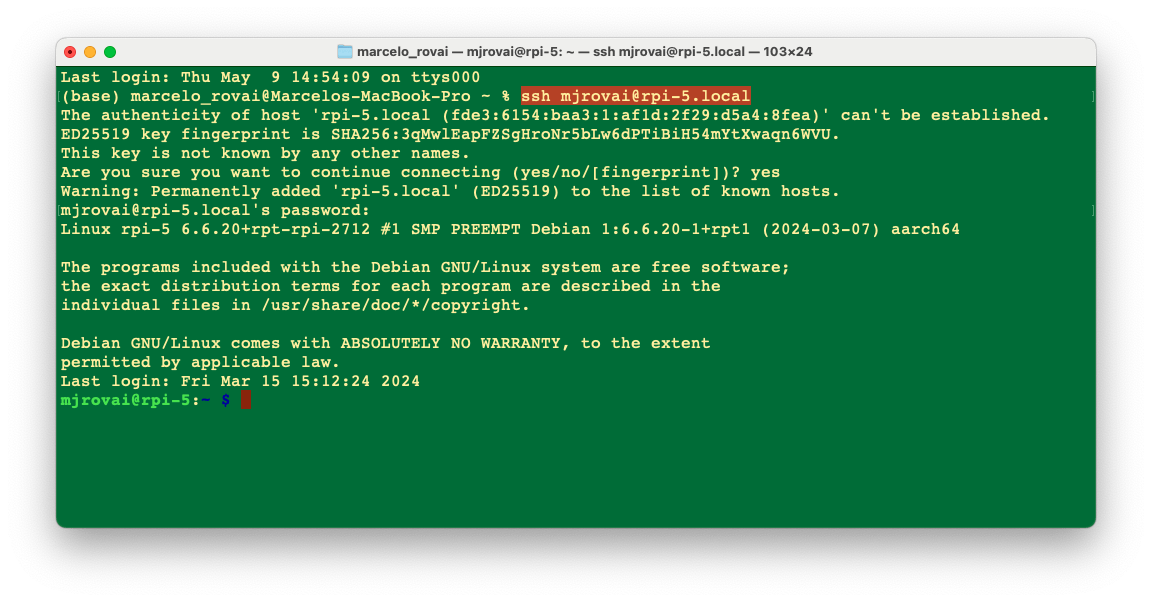
\includegraphics[width=0.85\linewidth,height=\textheight,keepaspectratio]{images/png/ssh.png}

  }

  \caption{img}

  \end{figure}%

  When you see the prompt:

\begin{Shaded}
\begin{Highlighting}[]
\ExtensionTok{mjrovai@rpi{-}5:\textasciitilde{}}\NormalTok{ $}
\end{Highlighting}
\end{Shaded}

  It means that you are interacting remotely with your Raspi. It is a
  good practice to update/upgrade the system regularly. For that, you
  should run:

\begin{Shaded}
\begin{Highlighting}[]
\FunctionTok{sudo}\NormalTok{ apt{-}get update}
\FunctionTok{sudo}\NormalTok{ apt upgrade}
\end{Highlighting}
\end{Shaded}

  You should confirm the Raspi IP address. On the terminal, you can use:

\begin{Shaded}
\begin{Highlighting}[]
\FunctionTok{hostname} \AttributeTok{{-}I}
\end{Highlighting}
\end{Shaded}
\end{enumerate}

\noindent \begin{center}
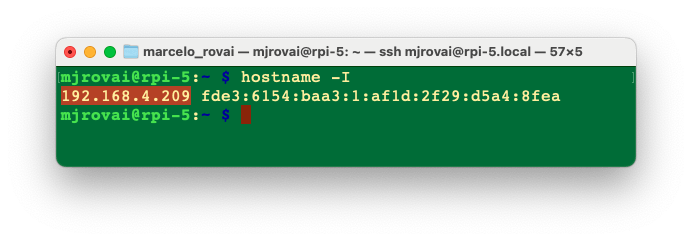
\includegraphics[width=0.85\linewidth,height=\textheight,keepaspectratio]{images/png/pasted_graphic_11_ilcmyoyu7x.png}
\end{center}

\subsubsection{To shut down the Raspi via
terminal:}\label{sec-setup-shut-raspi-via-terminal-c248}

When you want to turn off your Raspberry Pi, there are better ideas than
just pulling the power cord. This is because the Raspi may still be
writing data to the SD card, in which case merely powering down may
result in data loss or, even worse, a corrupted SD card.

For safety shut down, use the command line:

\begin{Shaded}
\begin{Highlighting}[]
\FunctionTok{sudo}\NormalTok{ shutdown }\AttributeTok{{-}h}\NormalTok{ now}
\end{Highlighting}
\end{Shaded}

\begin{quote}
To avoid possible data loss and SD card corruption, before removing the
power, you should wait a few seconds after shutdown for the Raspberry
Pi's LED to stop blinking and go dark. Once the LED goes out, it's safe
to power down.
\end{quote}

\subsubsection{Transfer Files between the Raspi and a
computer}\label{sec-setup-transfer-files-raspi-computer-77e4}

Transferring files between the Raspi and our main computer can be done
using a pen drive, directly on the terminal (with scp), or an FTP
program over the network.

\paragraph{\texorpdfstring{Using Secure Copy Protocol
(\texttt{scp}):}{Using Secure Copy Protocol (scp):}}\label{sec-setup-using-secure-copy-protocol-scp-310d}

\subparagraph{Copy files to your Raspberry
Pi}\label{sec-setup-copy-files-raspberry-pi-1a8b}

Let's create a text file on our computer, for example,
\texttt{test.txt}.

\noindent \begin{center}
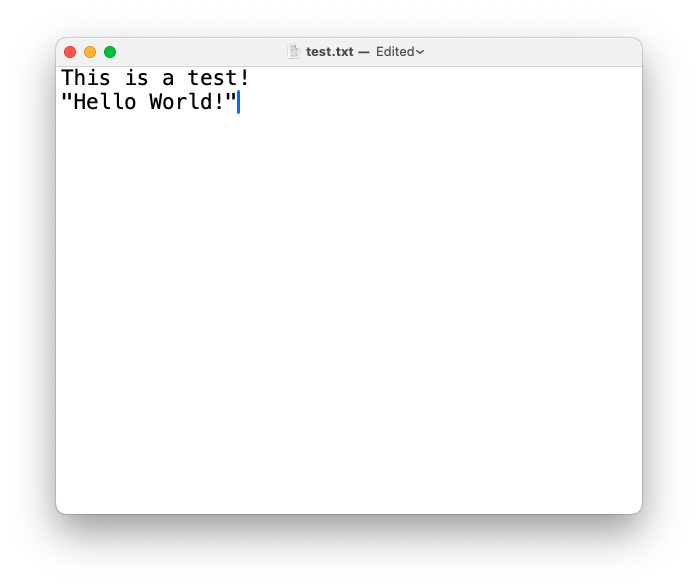
\includegraphics[width=0.7\linewidth,height=\textheight,keepaspectratio]{images/png/test_txt.png}
\end{center}

\begin{quote}
You can use any text editor. In the same terminal, an option is the
\texttt{nano}.
\end{quote}

To copy the file named \texttt{test.txt} from your personal computer to
a user's home folder on your Raspberry Pi, run the following command
from the directory containing \texttt{test.txt}, replacing the
\texttt{\textless{}username\textgreater{}} placeholder with the username
you use to log in to your Raspberry Pi and the
\texttt{\textless{}pi\_ip\_address\textgreater{}} placeholder with your
Raspberry Pi's IP address:

\begin{Shaded}
\begin{Highlighting}[]
\ExtensionTok{$}\NormalTok{ scp test.txt }\OperatorTok{\textless{}}\NormalTok{username}\OperatorTok{\textgreater{}}\NormalTok{@}\OperatorTok{\textless{}}\NormalTok{pi\_ip\_address}\OperatorTok{\textgreater{}}\NormalTok{:\textasciitilde{}/}
\end{Highlighting}
\end{Shaded}

\begin{quote}
Note that \texttt{\textasciitilde{}/} means that we will move the file
to the ROOT of our Raspi. You can choose any folder in your Raspi. But
you should create the folder before you run \texttt{scp}, since
\texttt{scp} won't create folders automatically.
\end{quote}

For example, let's transfer the file \texttt{test.txt} to the ROOT of my
Raspi-zero, which has an IP of \texttt{192.168.4.210}:

\begin{Shaded}
\begin{Highlighting}[]
\FunctionTok{scp}\NormalTok{ test.txt mjrovai@192.168.4.210:\textasciitilde{}/}
\end{Highlighting}
\end{Shaded}

\noindent
\pandocbounded{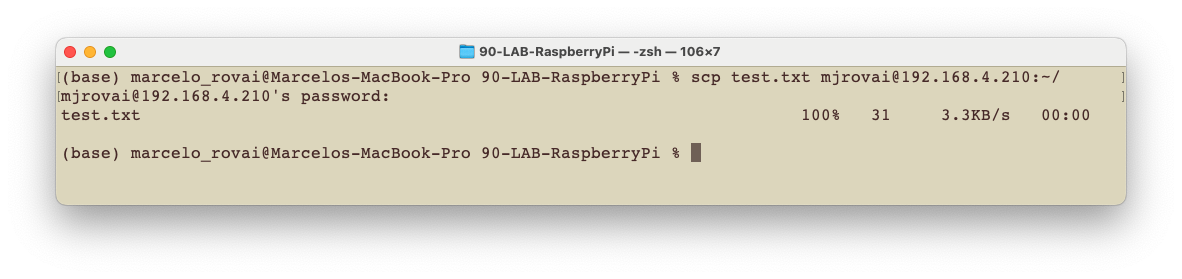
\includegraphics[keepaspectratio]{images/png/transfer_file.png}}

I use a different profile to differentiate the terminals. The above
action happens \textbf{on your computer}. Now, let's go to our Raspi
(using the SSH) and check if the file is there:

\noindent
\pandocbounded{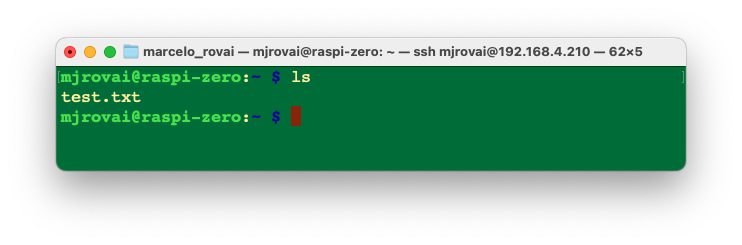
\includegraphics[keepaspectratio]{images/png/list_archives.png}}

\subparagraph{Copy files from your Raspberry
Pi}\label{sec-setup-copy-files-raspberry-pi-db9b}

To copy a file named \texttt{test.txt} from a user's home directory on a
Raspberry Pi to the current directory on another computer, run the
following command \textbf{on your Host Computer}:

\begin{Shaded}
\begin{Highlighting}[]
\ExtensionTok{$}\NormalTok{ scp }\OperatorTok{\textless{}}\NormalTok{username}\OperatorTok{\textgreater{}}\NormalTok{@}\OperatorTok{\textless{}}\NormalTok{pi\_ip\_address}\OperatorTok{\textgreater{}}\NormalTok{:myfile.txt .}
\end{Highlighting}
\end{Shaded}

For example:

On the Raspi, let's create a copy of the file with another name:

\begin{Shaded}
\begin{Highlighting}[]
\FunctionTok{cp}\NormalTok{ test.txt test\_2.txt}
\end{Highlighting}
\end{Shaded}

And on the Host Computer (in my case, a Mac)

\begin{Shaded}
\begin{Highlighting}[]
\FunctionTok{scp}\NormalTok{ mjrovai@192.168.4.210:test\_2.txt .}
\end{Highlighting}
\end{Shaded}

\noindent
\pandocbounded{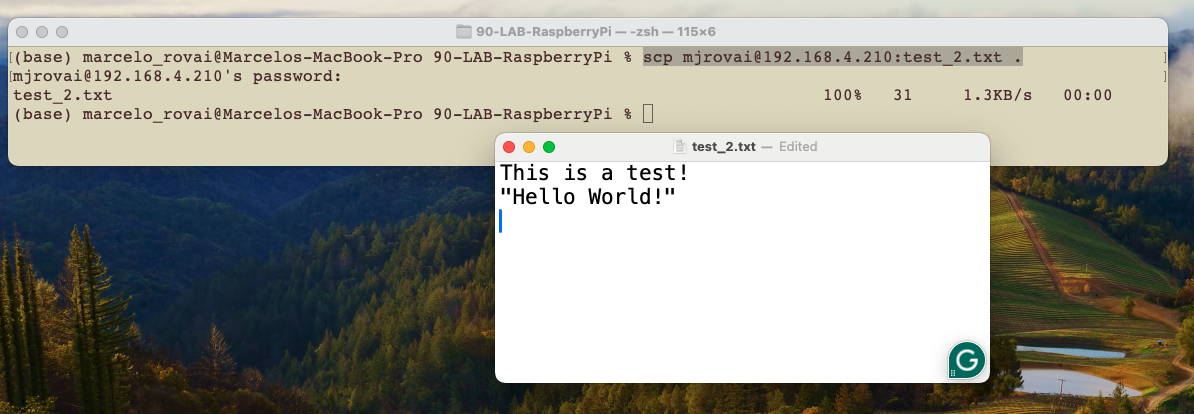
\includegraphics[keepaspectratio]{images/png/tranfer-text-mac.png}}

\paragraph{Transferring files using
FTP}\label{sec-setup-transferring-files-using-ftp-9310}

Transferring files using FTP, such as
\href{https://filezilla-project.org/download.php?type=client}{FileZilla
FTP Client}, is also possible. Follow the instructions, install the
program for your Desktop OS, and use the Raspi IP address as the
\texttt{Host}. For example:

\begin{Shaded}
\begin{Highlighting}[]
\ExtensionTok{sftp://192.168.4.210}
\end{Highlighting}
\end{Shaded}

\noindent and enter your Raspi \texttt{username\ and\ password}.
Pressing \texttt{Quickconnect} will open two windows, one for your host
computer desktop (right) and another for the Raspi (left).

\noindent \begin{center}
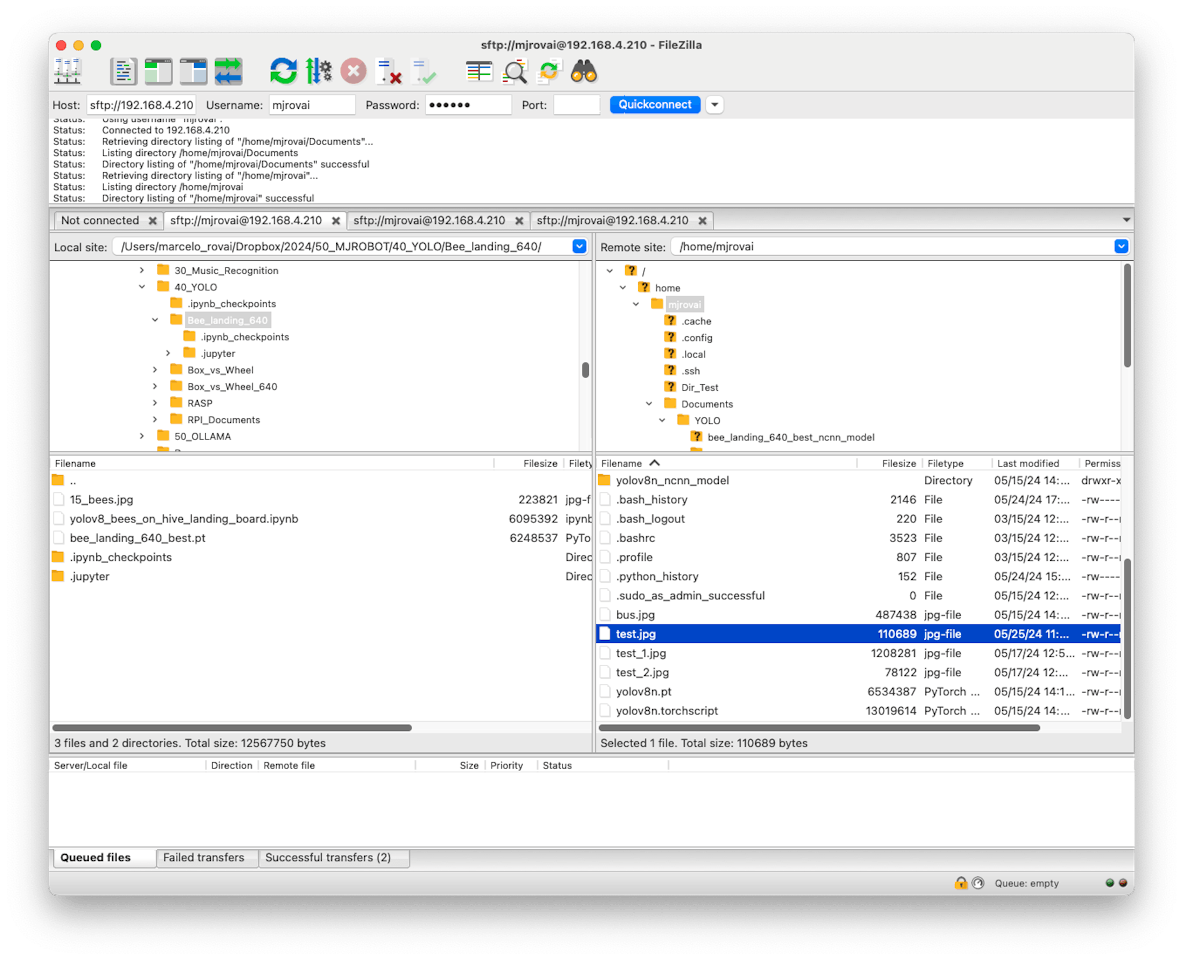
\includegraphics[width=0.8\linewidth,height=\textheight,keepaspectratio]{images/png/filezila.png}
\end{center}

\subsection{Increasing SWAP
Memory}\label{sec-setup-increasing-swap-memory-d591}

Using \texttt{htop}, a cross-platform interactive process viewer, you
can easily monitor the resources running on your Raspi, such as the list
of processes, the running CPUs, and the memory used in real-time. To
lunch \texttt{hop}, enter with the command on the terminal:

\begin{Shaded}
\begin{Highlighting}[]
\ExtensionTok{htop}
\end{Highlighting}
\end{Shaded}

\noindent \begin{center}
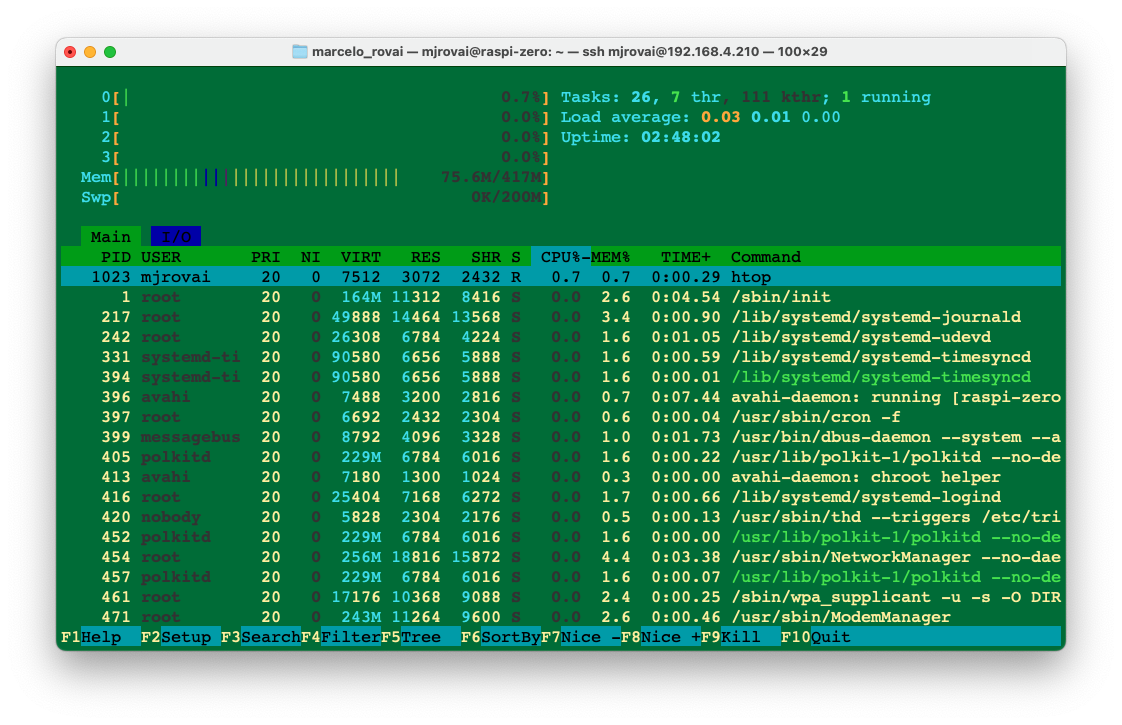
\includegraphics[width=0.8\linewidth,height=\textheight,keepaspectratio]{images/png/htop.png}
\end{center}

Regarding memory, among the devices in the Raspberry Pi family, the
Raspi-Zero has the smallest amount of SRAM (500 MB), compared to a
selection of 2 GB to 8 GB on the Raspis 4 or 5. For any Raspi, it is
possible to increase the memory available to the system with ``Swap.''
Swap memory, also known as swap space, is a technique used in computer
operating systems to temporarily store data from RAM (Random Access
Memory) on the SD card when the physical RAM is fully utilized. This
allows the operating system (OS) to continue running even when RAM is
full, which can prevent system crashes or slowdowns.

Swap memory benefits devices with limited RAM, such as the Raspi-Zero.
Increasing swap can help run more demanding applications or processes,
but it's essential to balance this with the potential performance impact
of frequent disk access.

By default, the Rapi-Zero's SWAP (Swp) memory is only 100 MB, which is
very small for running some more complex and demanding Machine Learning
applications (for example, YOLO). Let's increase it to 2 MB:

First, turn off swap-file:

\begin{Shaded}
\begin{Highlighting}[]
\FunctionTok{sudo}\NormalTok{ dphys{-}swapfile swapoff}
\end{Highlighting}
\end{Shaded}

Next, you should open and change the file \texttt{/etc/dphys-swapfile}.
For that, we will use the nano:

\begin{Shaded}
\begin{Highlighting}[]
\FunctionTok{sudo}\NormalTok{ nano /etc/dphys{-}swapfile}
\end{Highlighting}
\end{Shaded}

Search for the \textbf{CONF\_SWAPSIZE} variable (default is 200) and
update it to \textbf{2000}:

\begin{Shaded}
\begin{Highlighting}[]
\VariableTok{CONF\_SWAPSIZE}\OperatorTok{=}\NormalTok{2000}
\end{Highlighting}
\end{Shaded}

And save the file.

Next, turn on the swapfile again and reboot the Raspi-zero:

\begin{Shaded}
\begin{Highlighting}[]
\FunctionTok{sudo}\NormalTok{ dphys{-}swapfile setup}
\FunctionTok{sudo}\NormalTok{ dphys{-}swapfile swapon}
\FunctionTok{sudo}\NormalTok{ reboot}
\end{Highlighting}
\end{Shaded}

When your device is rebooted (you should enter with the SSH again), you
will realize that the maximum swap memory value shown on top is now
something near 2 GB (in my case, 1.95 GB).

\begin{quote}
To keep the \emph{htop} running, you should open another terminal window
to interact continuously with your Raspi.
\end{quote}

\subsection{Installing a Camera}\label{sec-setup-installing-camera-403e}

The Raspi is an excellent device for computer vision applications; a
camera is needed for it. We can install a standard USB webcam on the
micro-USB port using a USB OTG adapter (Raspi-Zero and Raspi-5) or a
camera module connected to the Raspi CSI (Camera Serial Interface) port.

\begin{quote}
USB Webcams generally have inferior quality to the camera modules that
connect to the CSI port. They can also not be controlled using the
\texttt{raspistill} and \texttt{raspivid} commands in the terminal or
the \texttt{picamera} recording package in Python. Nevertheless, there
may be reasons why you want to connect a USB camera to your Raspberry
Pi, such as because of the benefit that it is much easier to set up
multiple cameras with a single Raspberry Pi, long cables, or simply
because you have such a camera on hand.
\end{quote}

\subsubsection{Installing a USB
WebCam}\label{sec-setup-installing-usb-webcam-2569}

\begin{enumerate}
\def\labelenumi{\arabic{enumi}.}
\tightlist
\item
  Power off the Raspi:
\end{enumerate}

\begin{Shaded}
\begin{Highlighting}[]
\FunctionTok{sudo}\NormalTok{ shutdown }\AttributeTok{{-}h}\NormalTok{ no}
\end{Highlighting}
\end{Shaded}

\begin{enumerate}
\def\labelenumi{\arabic{enumi}.}
\setcounter{enumi}{1}
\tightlist
\item
  Connect the USB Webcam (USB Camera Module 30 fps, \(1280\times 720\))
  to your Raspi (In this example, I am using the Raspi-Zero, but the
  instructions work for all Raspis).
\end{enumerate}

\noindent \begin{center}
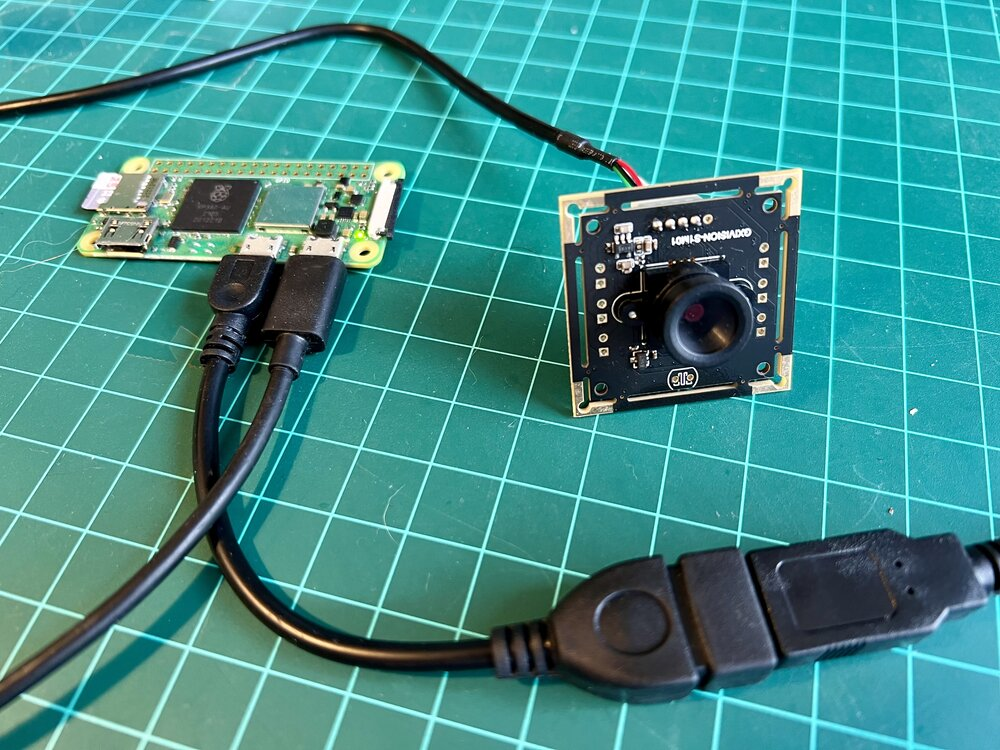
\includegraphics[width=0.95\linewidth,height=\textheight,keepaspectratio]{images/jpeg/usb-cam-2.jpg}
\end{center}

\begin{enumerate}
\def\labelenumi{\arabic{enumi}.}
\setcounter{enumi}{2}
\tightlist
\item
  Power on again and run the SSH
\item
  To check if your USB camera is recognized, run:
\end{enumerate}

\begin{Shaded}
\begin{Highlighting}[]
\ExtensionTok{lsusb}
\end{Highlighting}
\end{Shaded}

You should see your camera listed in the output.

\noindent \begin{center}
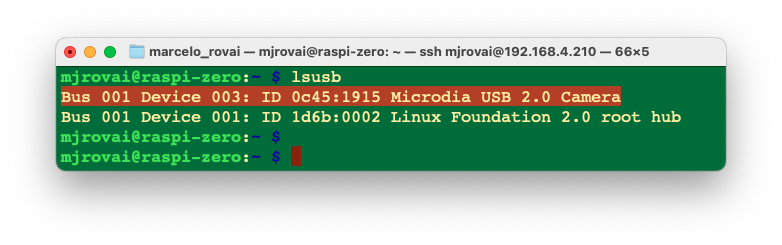
\includegraphics[width=0.75\linewidth,height=\textheight,keepaspectratio]{images/png/usb-cam-2.png}
\end{center}

\begin{enumerate}
\def\labelenumi{\arabic{enumi}.}
\setcounter{enumi}{4}
\tightlist
\item
  To take a test picture with your USB camera, use:
\end{enumerate}

\begin{Shaded}
\begin{Highlighting}[]
\ExtensionTok{fswebcam}\NormalTok{ test\_image.jpg}
\end{Highlighting}
\end{Shaded}

This will save an image named ``test\_image.jpg'' in your current
directory.

\noindent \begin{center}
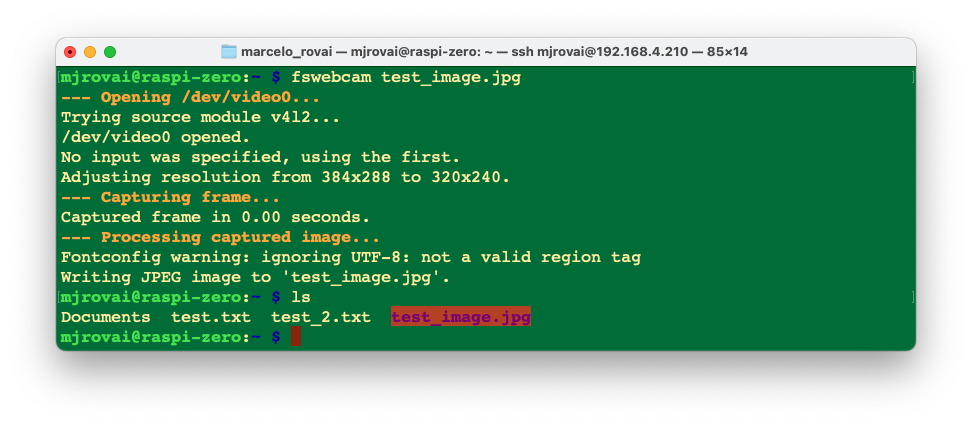
\includegraphics[width=0.85\linewidth,height=\textheight,keepaspectratio]{images/png/image-test.png}
\end{center}

\begin{enumerate}
\def\labelenumi{\arabic{enumi}.}
\setcounter{enumi}{5}
\tightlist
\item
  Since we are using SSH to connect to our Rapsi, we must transfer the
  image to our main computer so we can view it. We can use FileZilla or
  SCP for this:
\end{enumerate}

Open a terminal \textbf{on your host computer} and run:

\begin{Shaded}
\begin{Highlighting}[]
\FunctionTok{scp}\NormalTok{ mjrovai@raspi{-}zero.local:\textasciitilde{}/test\_image.jpg .}
\end{Highlighting}
\end{Shaded}

\begin{quote}
Replace ``mjrovai'' with your username and ``raspi-zero'' with Pi's
hostname.
\end{quote}

\noindent \begin{center}
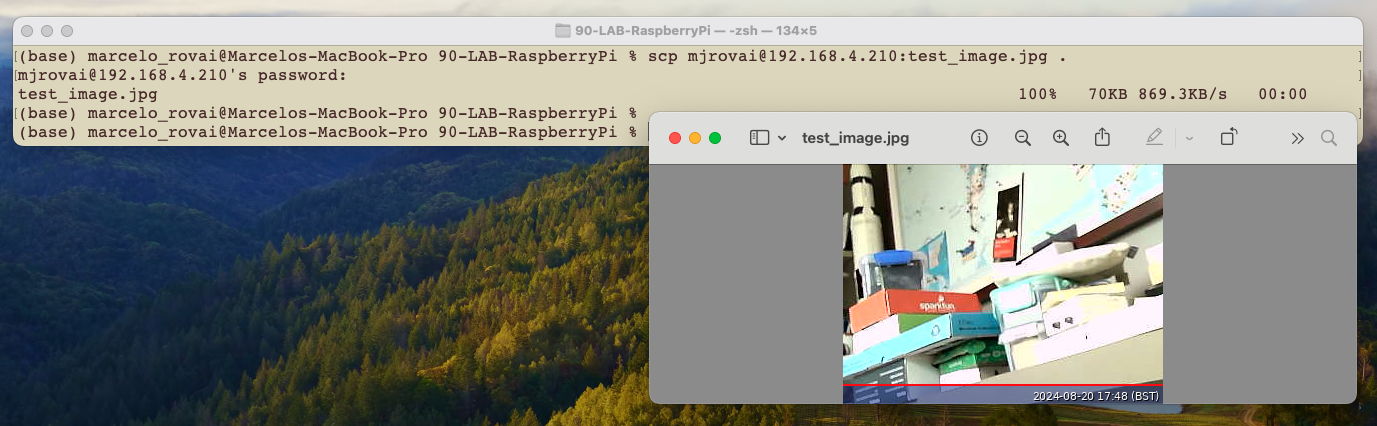
\includegraphics[width=0.8\linewidth,height=\textheight,keepaspectratio]{images/png/cam-2_test.png}
\end{center}

\begin{enumerate}
\def\labelenumi{\arabic{enumi}.}
\setcounter{enumi}{6}
\tightlist
\item
  If the image quality isn't satisfactory, you can adjust various
  settings; for example, define a resolution that is suitable for YOLO
  \((640x640)\):
\end{enumerate}

\begin{Shaded}
\begin{Highlighting}[]
\ExtensionTok{fswebcam} \AttributeTok{{-}r}\NormalTok{ 640x640 }\AttributeTok{{-}{-}no{-}banner}\NormalTok{ test\_image\_yolo.jpg}
\end{Highlighting}
\end{Shaded}

This captures a higher-resolution image without the default banner.

\noindent \begin{center}
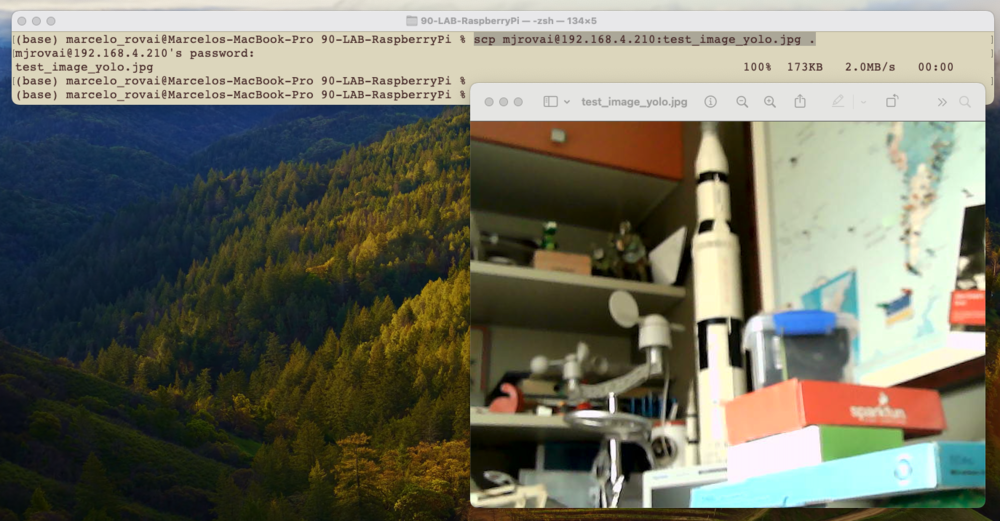
\includegraphics[width=0.85\linewidth,height=\textheight,keepaspectratio]{images/png/usb-cam-test-2.png}
\end{center}

An ordinary USB Webcam can also be used:

\noindent \begin{center}
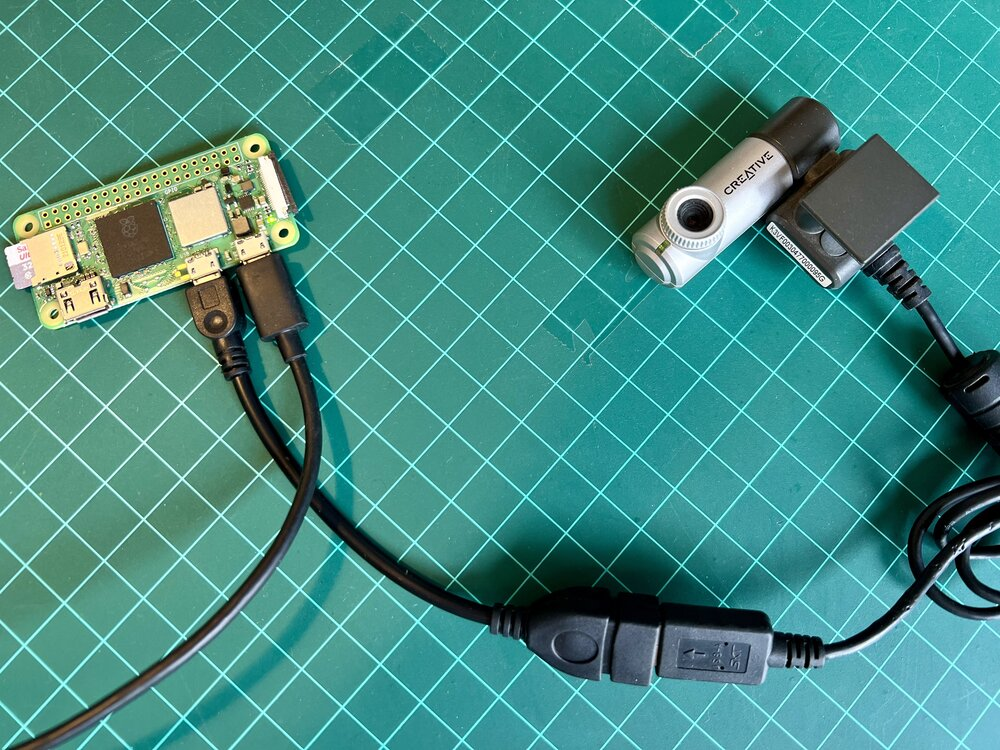
\includegraphics[width=0.85\linewidth,height=\textheight,keepaspectratio]{images/jpeg/usb_camera.jpg}
\end{center}

And verified using \texttt{lsusb}

\noindent
\pandocbounded{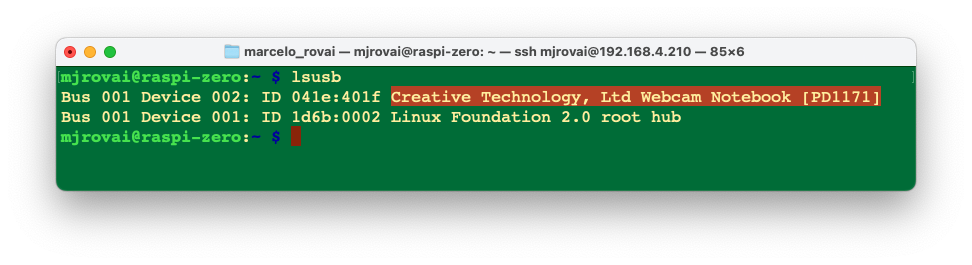
\includegraphics[keepaspectratio]{images/png/usb-cam-test.png}}

\paragraph{Video Streaming}\label{sec-setup-video-streaming-e1a8}

For stream video (which is more resource-intensive), we can install and
use mjpg-streamer:

First, install Git:

\begin{Shaded}
\begin{Highlighting}[]
\FunctionTok{sudo}\NormalTok{ apt install git}
\end{Highlighting}
\end{Shaded}

Now, we should install the necessary dependencies for mjpg-streamer,
clone the repository, and proceed with the installation:

\begin{Shaded}
\begin{Highlighting}[]
\FunctionTok{sudo}\NormalTok{ apt install cmake libjpeg62{-}turbo{-}dev}
\FunctionTok{git}\NormalTok{ clone https://github.com/jacksonliam/mjpg{-}streamer.git}
\BuiltInTok{cd}\NormalTok{ mjpg{-}streamer/mjpg{-}streamer{-}experimental}
\FunctionTok{make}
\FunctionTok{sudo}\NormalTok{ make install}
\end{Highlighting}
\end{Shaded}

Then start the stream with:

\begin{Shaded}
\begin{Highlighting}[]
\ExtensionTok{mjpg\_streamer} \AttributeTok{{-}i} \StringTok{"input\_uvc.so"} \AttributeTok{{-}o} \StringTok{"output\_http.so {-}w ./www"}
\end{Highlighting}
\end{Shaded}

We can then access the stream by opening a web browser and navigating
to:

\texttt{http://\textless{}your\_pi\_ip\_address\textgreater{}:8080}. In
my case: http://192.168.4.210:8080

We should see a webpage with options to view the stream. Click on the
link that says ``Stream'' or try accessing:

\begin{Shaded}
\begin{Highlighting}[]
\ExtensionTok{http://}\OperatorTok{\textless{}}\NormalTok{raspberry\_pi\_ip\_address}\OperatorTok{\textgreater{}}\NormalTok{:8080/}\PreprocessorTok{?}\NormalTok{action=stream}
\end{Highlighting}
\end{Shaded}

\noindent
\pandocbounded{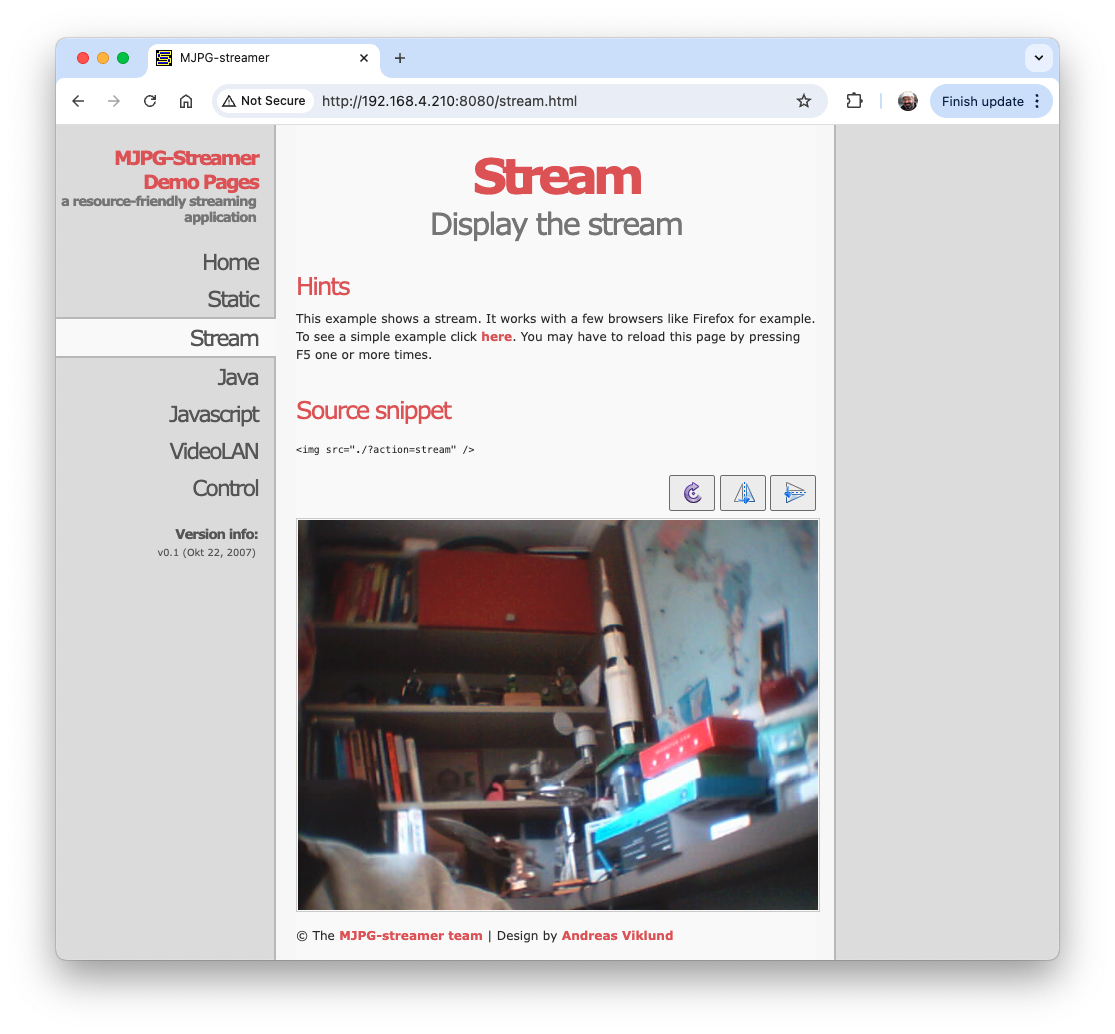
\includegraphics[keepaspectratio]{images/png/stream.png}}

\subsubsection{Installing a Camera Module on the CSI
port}\label{sec-setup-installing-camera-module-csi-port-13b9}

There are now several Raspberry Pi camera modules. The original
5-megapixel model was
\href{https://www.raspberrypi.com/news/camera-board-available-for-sale/}{released}
in 2013, followed by an
\href{https://www.raspberrypi.com/products/camera-module-v2/}{8-megapixel
Camera Module 2} that was later released in 2016. The latest camera
model is the
\href{https://www.raspberrypi.com/documentation/accessories/camera.html}{12-megapixel
Camera Module 3}, released in 2023.

The original 5 MP camera (\textbf{Arducam OV5647}) is no longer
available from Raspberry Pi but can be found from several alternative
suppliers. Below is an example of such a camera on a Raspi-Zero.

\noindent
\pandocbounded{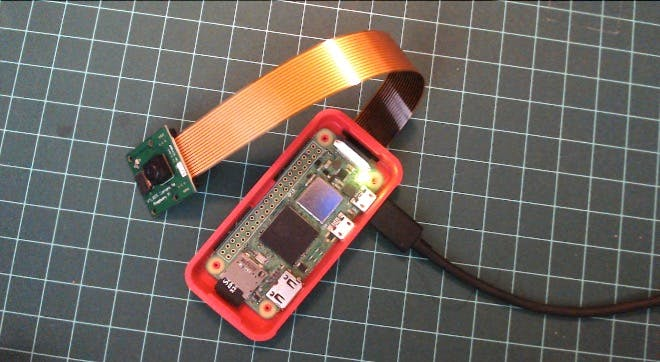
\includegraphics[keepaspectratio]{images/jpeg/rasp-zero-with-cam.jpg}}

Here is another example of a v2 Camera Module, which has a \textbf{Sony
IMX219} 8-megapixel sensor:

\noindent
\pandocbounded{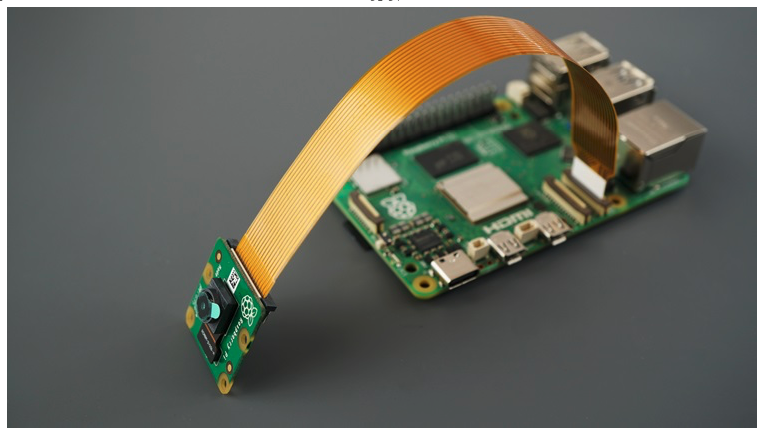
\includegraphics[keepaspectratio]{images/png/raspi-5-cam.png}}

Any camera module will work on the Raspberry Pis, but for that, the
\texttt{configuration.txt} file must be updated:

\begin{Shaded}
\begin{Highlighting}[]
\FunctionTok{sudo}\NormalTok{ nano /boot/firmware/config.txt}
\end{Highlighting}
\end{Shaded}

At the bottom of the file, for example, to use the 5 MP Arducam OV5647
camera, add the line:

\begin{Shaded}
\begin{Highlighting}[]
\VariableTok{dtoverlay}\OperatorTok{=}\NormalTok{ov5647,cam0}
\end{Highlighting}
\end{Shaded}

Or for the v2 module, which has the 8MP Sony IMX219 camera:

\begin{Shaded}
\begin{Highlighting}[]
\VariableTok{dtoverlay}\OperatorTok{=}\NormalTok{imx219,cam0}
\end{Highlighting}
\end{Shaded}

Save the file (CTRL+O {[}ENTER{]} CRTL+X) and reboot the Raspi:

\begin{Shaded}
\begin{Highlighting}[]
\ExtensionTok{Sudo}\NormalTok{ reboot}
\end{Highlighting}
\end{Shaded}

After the boot, you can see if the camera is listed:

\begin{Shaded}
\begin{Highlighting}[]
\ExtensionTok{libcamera{-}hello} \AttributeTok{{-}{-}list{-}cameras}
\end{Highlighting}
\end{Shaded}

\noindent
\pandocbounded{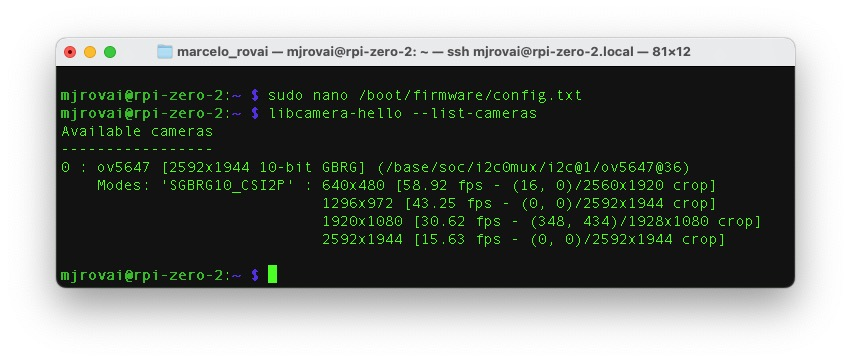
\includegraphics[keepaspectratio]{images/jpeg/list_cams_raspi-zero.jpg}}

\noindent
\pandocbounded{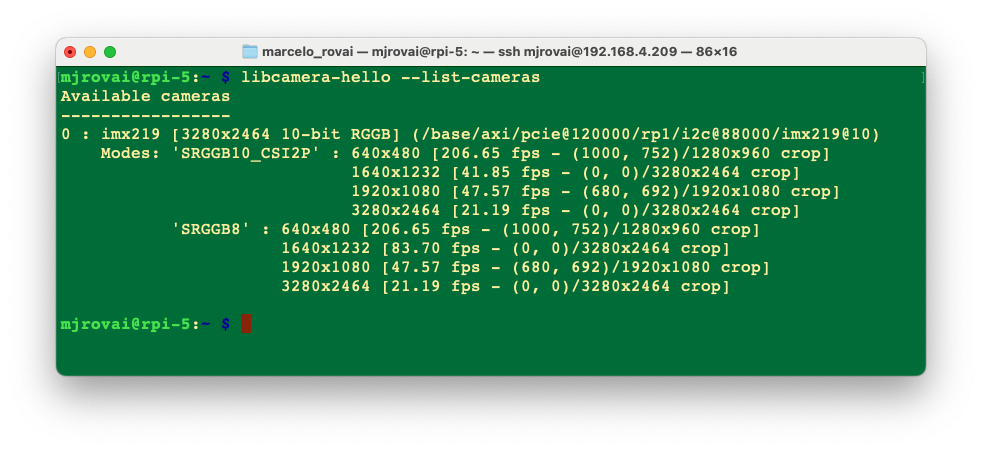
\includegraphics[keepaspectratio]{images/png/list_cams_raspi-5.png}}

\begin{quote}
\href{https://www.raspberrypi.com/documentation/computers/camera_software.html\#libcamera}{libcamera}
is an open-source software library that supports camera systems directly
from the Linux operating system on Arm processors. It minimizes
proprietary code running on the Broadcom GPU.
\end{quote}

Let's capture a jpeg image with a resolution of \(640\times 480\) for
testing and save it to a file named \texttt{test\_cli\_camera.jpg}

\begin{Shaded}
\begin{Highlighting}[]
\ExtensionTok{rpicam{-}jpeg} \AttributeTok{{-}{-}output}\NormalTok{ test\_cli\_camera.jpg }\AttributeTok{{-}{-}width}\NormalTok{ 640 }\AttributeTok{{-}{-}height}\NormalTok{ 480}
\end{Highlighting}
\end{Shaded}

\noindent if we want to see the file saved, we should use
\texttt{ls\ -f}, which lists all current directory content in long
format. As before, we can use scp to view the image:

\noindent \begin{center}
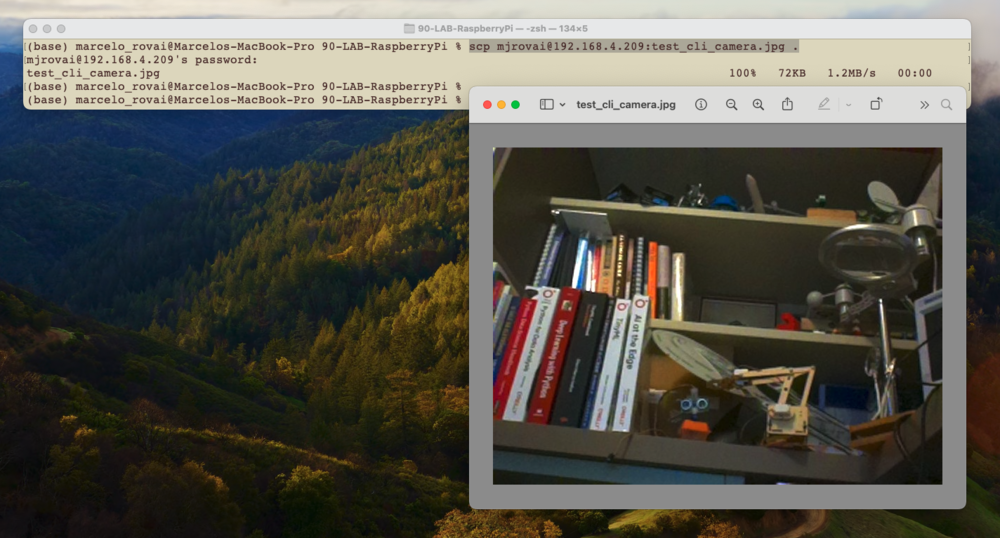
\includegraphics[width=0.85\linewidth,height=\textheight,keepaspectratio]{images/png/test_camera_raspi-5.png}
\end{center}

\subsection{Running the Raspi Desktop
remotely}\label{sec-setup-running-raspi-desktop-remotely-476c}

While we've primarily interacted with the Raspberry Pi using terminal
commands via SSH, we can access the whole graphical desktop environment
remotely if we have installed the complete Raspberry Pi OS (for example,
\texttt{Raspberry\ Pi\ OS\ (64-bit)}. This can be particularly useful
for tasks that benefit from a visual interface. To enable this
functionality, we must set up a VNC (Virtual Network Computing) server
on the Raspberry Pi. Here's how to do it:

\begin{enumerate}
\def\labelenumi{\arabic{enumi}.}
\tightlist
\item
  Enable the VNC Server:

  \begin{itemize}
  \item
    Connect to your Raspberry Pi via SSH.
  \item
    Run the Raspberry Pi configuration tool by entering:

\begin{Shaded}
\begin{Highlighting}[]
\FunctionTok{sudo}\NormalTok{ raspi{-}config}
\end{Highlighting}
\end{Shaded}
  \item
    Navigate to \texttt{Interface\ Options} using the arrow keys.
  \end{itemize}
\end{enumerate}

\noindent
\pandocbounded{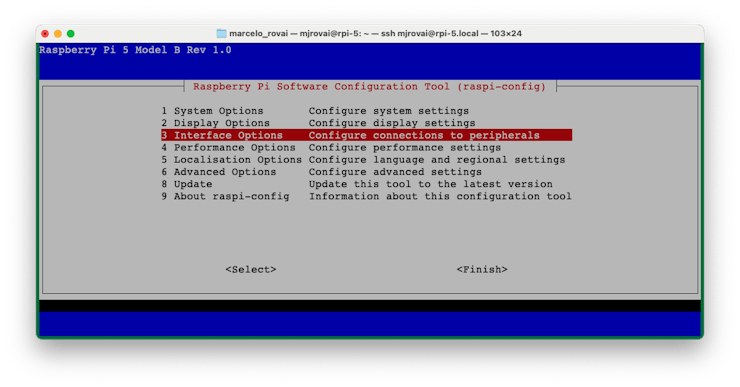
\includegraphics[keepaspectratio]{images/png/vnc-1.png}}

\begin{itemize}
\tightlist
\item
  Select \texttt{VNC} and \texttt{Yes} to enable the VNC server.
\end{itemize}

\noindent
\pandocbounded{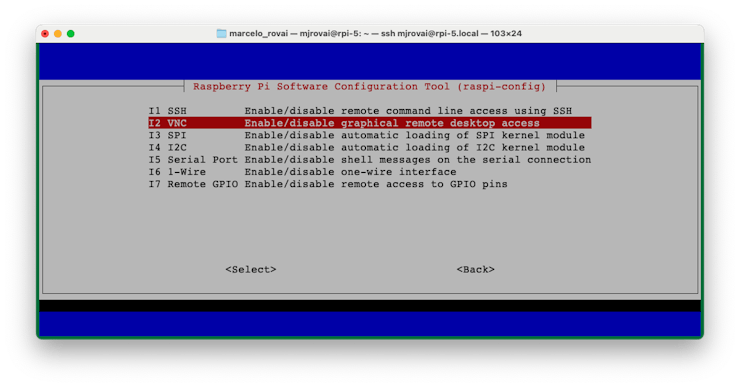
\includegraphics[keepaspectratio]{images/png/vnc-2.png}}

\begin{itemize}
\tightlist
\item
  Exit the configuration tool, saving changes when prompted.
\end{itemize}

\noindent
\pandocbounded{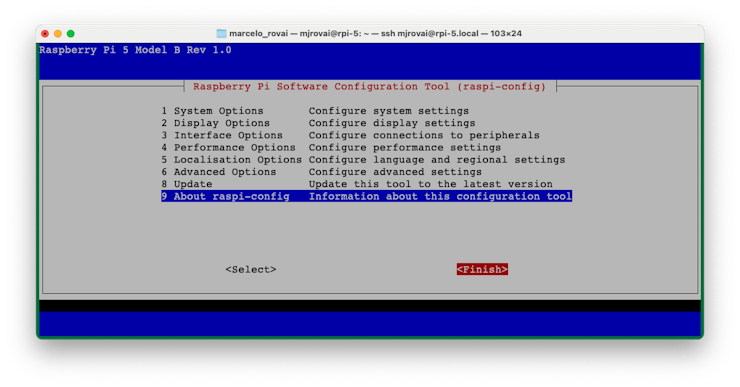
\includegraphics[keepaspectratio]{images/png/vnc-3.png}}

\begin{enumerate}
\def\labelenumi{\arabic{enumi}.}
\setcounter{enumi}{1}
\item
  Install a VNC Viewer on Your Computer:

  \begin{itemize}
  \tightlist
  \item
    Download and install a VNC viewer application on your main computer.
    Popular options include RealVNC Viewer, TightVNC, or VNC Viewer by
    RealVNC. We will install
    \href{https://www.realvnc.com/en/connect/download/viewer}{VNC
    Viewer} by RealVNC.
  \end{itemize}
\item
  Once installed, you should confirm the Raspi IP address. For example,
  on the terminal, you can use:

\begin{Shaded}
\begin{Highlighting}[]
\FunctionTok{hostname} \AttributeTok{{-}I}
\end{Highlighting}
\end{Shaded}
\end{enumerate}

\noindent \begin{center}
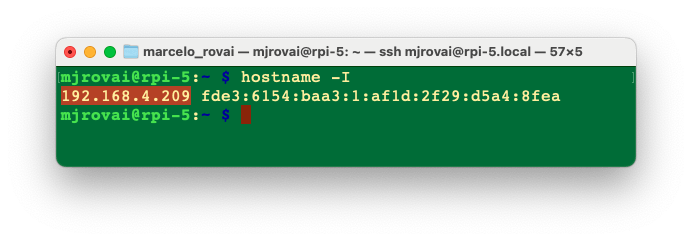
\includegraphics[width=0.85\linewidth,height=\textheight,keepaspectratio]{images/png/vnc-4.png}
\end{center}

\begin{enumerate}
\def\labelenumi{\arabic{enumi}.}
\setcounter{enumi}{3}
\tightlist
\item
  Connect to Your Raspberry Pi:

  \begin{itemize}
  \tightlist
  \item
    Open your VNC viewer application.
  \end{itemize}
\end{enumerate}

\noindent \begin{center}
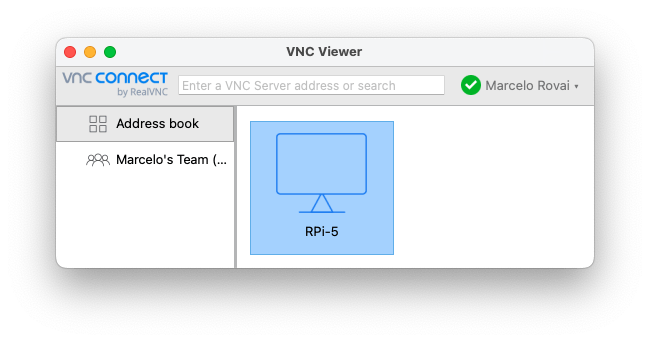
\includegraphics[width=0.85\linewidth,height=\textheight,keepaspectratio]{images/png/vnc-5.png}
\end{center}

\begin{itemize}
\tightlist
\item
  Enter your Raspberry Pi's IP address and hostname.
\item
  When prompted, enter your Raspberry Pi's username and password.
\end{itemize}

\noindent \begin{center}
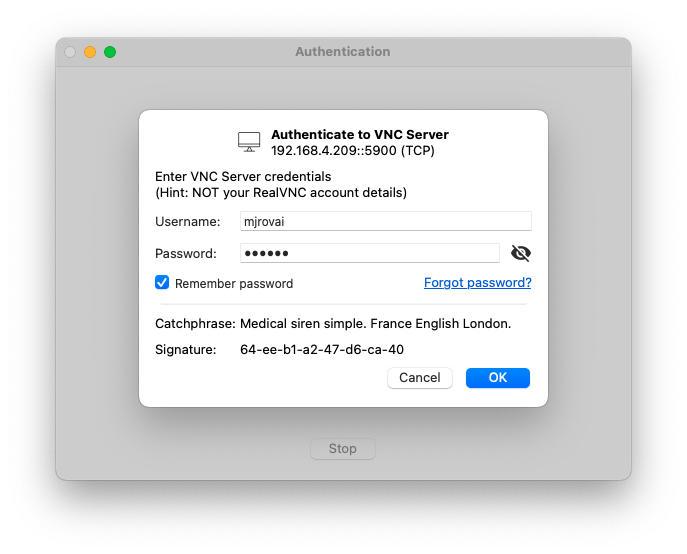
\includegraphics[width=0.8\linewidth,height=\textheight,keepaspectratio]{images/png/vnc-7.png}
\end{center}

\begin{enumerate}
\def\labelenumi{\arabic{enumi}.}
\setcounter{enumi}{4}
\tightlist
\item
  The Raspberry Pi 5 Desktop should appear on your computer monitor.
\end{enumerate}

\noindent \begin{center}
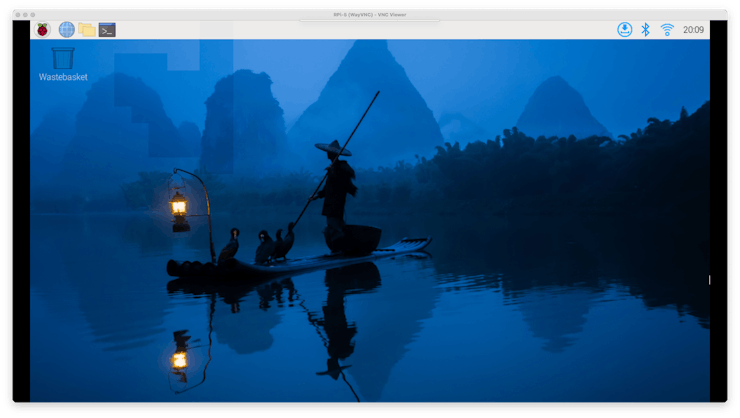
\includegraphics[width=0.85\linewidth,height=\textheight,keepaspectratio]{images/png/vnc-8.png}
\end{center}

\begin{enumerate}
\def\labelenumi{\arabic{enumi}.}
\setcounter{enumi}{5}
\item
  Adjust Display Settings (if needed):

  \begin{itemize}
  \tightlist
  \item
    Once connected, adjust the display resolution for optimal viewing.
    This can be done through the Raspberry Pi's desktop settings or by
    modifying the config.txt file.
  \item
    Let's do it using the desktop settings. Reach the menu (the
    Raspberry Icon at the left upper corner) and select the best screen
    definition for your monitor:
  \end{itemize}
\end{enumerate}

\noindent \begin{center}
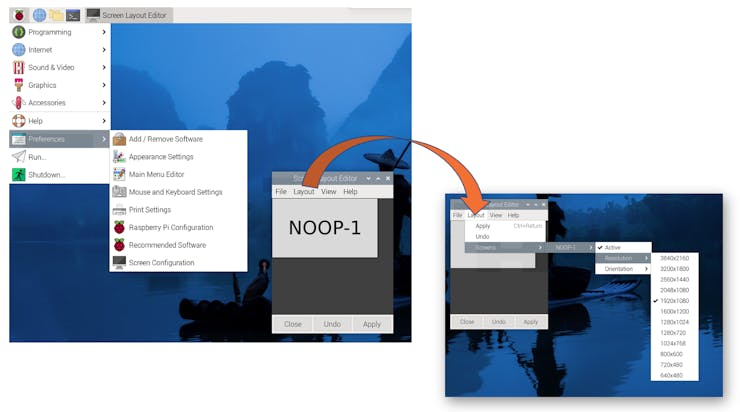
\includegraphics[width=0.9\linewidth,height=\textheight,keepaspectratio]{images/png/vnc-9.png}
\end{center}

\subsection{Updating and Installing
Software}\label{sec-setup-updating-installing-software-b85d}

\begin{enumerate}
\def\labelenumi{\arabic{enumi}.}
\item
  Update your system:

\begin{Shaded}
\begin{Highlighting}[]
\FunctionTok{sudo}\NormalTok{ apt update }\KeywordTok{\&\&} \FunctionTok{sudo}\NormalTok{ apt upgrade }\AttributeTok{{-}y}
\end{Highlighting}
\end{Shaded}
\item
  Install essential software:

\begin{Shaded}
\begin{Highlighting}[]
\FunctionTok{sudo}\NormalTok{ apt install python3{-}pip }\AttributeTok{{-}y}
\end{Highlighting}
\end{Shaded}
\item
  Enable pip for Python projects:

\begin{Shaded}
\begin{Highlighting}[]
\FunctionTok{sudo}\NormalTok{ rm /usr/lib/python3.11/EXTERNALLY{-}MANAGED}
\end{Highlighting}
\end{Shaded}
\end{enumerate}

\subsection{Model-Specific
Considerations}\label{sec-setup-modelspecific-considerations-8f09}

\subsubsection{Raspberry Pi Zero
(Raspi-Zero)}\label{sec-setup-raspberry-pi-zero-raspizero-f33d}

\begin{itemize}
\tightlist
\item
  Limited processing power, best for lightweight projects
\item
  It is better to use a headless setup (SSH) to conserve resources.
\item
  Consider increasing swap space for memory-intensive tasks.
\item
  It can be used for Image Classification and Object Detection Labs but
  not for the LLM (SLM).
\end{itemize}

\subsubsection{Raspberry Pi 4 or 5 (Raspi-4 or
Raspi-5)}\label{sec-setup-raspberry-pi-4-5-raspi4-raspi5-d816}

\begin{itemize}
\tightlist
\item
  Suitable for more demanding projects, including AI and machine
  learning.
\item
  It can run the whole desktop environment smoothly.
\item
  Raspi-4 can be used for Image Classification and Object Detection Labs
  but will not work well with LLMs (SLM).
\item
  For Raspi-5, consider using an active cooler for temperature
  management during intensive tasks, as in the LLMs (SLMs) lab.
\end{itemize}

Remember to adjust your project requirements based on the specific
Raspberry Pi model you're using. The Raspi-Zero is great for low-power,
space-constrained projects, while the Raspi-4 or 5 models are better
suited for more computationally intensive tasks.




\end{document}
